\chapter{Proteomic Characterization of Affinity-Purified Arabidopsis Proteasome Particles Identifies Sub-Complex Specific Interactors}

\section{Statement of Attribution}
Initial mutant characterization of \textit{rpt4} mutants was performed by Drs. Kwang-Hee Lee and Richard S. Marshall, postdoctoral fellows in the Vierstra Lab. Additionally, Dr. Lee generated the 2XFLAG-RPT4b transgenic line in the \textit{rpt4b-2} background.  I created the 2XFLAG-RPT4a \textit{rpt4a-1} transgenic lines. I developed the affinity purification via the RP with minor modifications from \citep{book10} by changing the primary buffer to HEPES. All mass-spectrometry sample preparation and data analysis in this chapter was completed by myself.  The actual running of the mass spectrometer was either performed by Dr. Mark Scalf in Dr. Lloyd M. Smith’s lab (Department of Chemistry, University of Wisconsin – Madison), or by Dr. Fionn McLoughlin in the Vierstra lab at Washington University.  I cloned the CP interactors PAP1, PBAC1, PBAC2, PBAC3, and PBAC4, and performed yeast-two-hybrid (Y2H) analysis on these.  While the streaking and yeast transformations were accomplished by myself, Dr. Marshall performed the final spotting of the yeast-two hybrid.  All BiFC data was generated by myself.  The HA-PAP1 transgenic line was created by Dr. Adam Book.  I developed the affinity purification for HA-PAP1 and performed the immunoblot analyses.  Native PAGE was performed by Dr. Marshall. \\


\noindent
We intend to submit this chapter to J. Biol. Chem. for publication as a research article in the near future.  A suggested list of authors is as follows: David Gemperline, Richard S. Marshall, Kwang-Hee Lee, Fionn McLoughlin, Mark Scalf, Lloyd M. Smith, and Richard D. Vierstra. 

\section{Abstract}

	The 26S proteasome is an ATP-dependent protease complex responsible for the selective removal of numerous eukaryotic proteins following their modification with polyubiquitin chains.  It consists of two sub-complexes, a self-compartmentalized core protease (CP) that degrades polypeptides within a central chamber, and a regulatory particle (RP) that caps one or both ends of the CP and is responsible for recognizing and unfolding ubiquitylated substrates, and transporting them into the CP lumen.  Previous mass spectrometric (MS) analyses of \textit{Arabidopsis} 26S proteasomes affinity-purified via the CP subunit PAG1 ($\alpha$7), detected a complex assortment of particles that are assembled using paired isoforms for many of the 33 core subunits, as well as a small assortment of associated factors that might help in assembly, regulation, substrate specificity, and ubiquitin recycling.  Here, we extended these studies by affinity purifying \textit{Arabidopsis} 26S proteasomes with either tagged isoform of the RP subunit RPT4 (named RPT4a and RPT4b).  Label-free quantitative (LFQ) MS analyses of the preparations detected both isoforms for many of the other CP and RP subunits, suggesting that plants incorporate subunit isoforms randomly into the holo-protease.  We also identified an array of interacting factors, including likely orthologs of the yeast assembly chaperones Ump1 and Pba1-4 for the CP, and Nas2, Nas6, and Hsm3 for the RP.  We additionally identified a novel plant-specific protein bound to the CP that interacts with the putative \textit{Arabidopsis} Pba1 ortholog, and possibly contributes to CP assembly.  By coupling native PAGE and MS analysis with proteasome preparations isolated from proteasome inhibitor-treated seedlings, we identified several assembly intermediates also harboring assembly chaperones and the proteasome regulators PA200 and ECM29.  Taken together these data suggest that \textit{Arabidopsis}, like yeast, dynamically employ a suite of assembly factors to construct the mature 26S particle.
 
\section{Introduction}
	The selective removal of proteins that are non-functional or have key regulatory roles is essential to normal plant growth and development. A major pathway for this selective removal is the ubiquitin 26S proteasome system, in which target proteins are covalently modified with the 76-amino-acid polypeptide ubiquitin and subsequently degraded by the central enzymatic effector in this process, the 26S proteasome (reviewed in \citep{finley09, livneh16, vierstra09}). The 26S proteasome consists of two major sub-complexes, the core protease (CP), which is responsible for degrading the substrate, and the regulatory particle (RP), which caps the CP at one or both ends and is responsible for recognizing and unfolding ubiquitylated substrates. Compositionally, the CP is made up of 28 subunits configured into four stacked hetero-heptameric rings made up of $\alpha$ and $\beta$-subunits in an $\alpha$1-7/$\beta$1-7/$\beta$1-7/$\alpha$1-7 arrangement. The N-termini of the $\beta$1, $\beta$2, and $\beta$5 subunits are enclosed in a central chamber by the surrounding $\alpha$-subunits, and together these $\beta$-subunits provide peptidylglutamyl-peptide-hydrolyzing activity ($\beta$1), trypsin-like ($\beta$2), and chymotrypsin-like ($\beta$5) activities. The $\alpha$-subunits possess N-terminal extensions that gate entry to the chamber, forming an axial pore that is only opened when substrates are actively processed by an associated RP, or when activated by alternative capping particles such as PA200 \citep{dange11, sadre-bazzaz10}.
	
The RP consists of two major sub-classes of proteins including six related AAA-ATPase (RPT) subunits (RPT1-6) and at least 15 non-AAA-ATPase (RPN) subunits (RPN1-3, 5-13, and SEM1) \citep{finley09, paraskevopoulos14, russell13}. The RPT subunits form a six-membered RPT ring responsible for unfolding the polypeptide substrate in an ATP dependent manner, and channeling the substrate through the axial pore into the central CP chamber. The RPN subunits have several differing functions including binding ubiquitylated substrates (RPN1, RPN10, RPN13, and SEM1 \citep{elsasser04, paraskevopoulos14, schreiner08, shi16}), binding ubiquitin shuttle proteins such as DSK2 and RAD23 \citep{elsasser02, farmer10, fatimababy10, lin11}, and releasing ubiquitin bound to substrates through the de-ubiquitylating activity of RPN11 \citep{verma02, yao02}.  RPN5-7 and RPN9 form a glove-like structure around the RPT ring providing structural support for adjacent subunits \citep{lander12, lasker12, unverdorben14}, with RPN6 acting as a molecular clamp that holds the RP and CP together \citep{pathare12}.

Over the last several years, analyses of the plant 26S proteasome have also revealed insights into its composition. Searches of the \textit{Arabidopsis} genome showed that plants typically encode two paralogs for most proteasome subunits \citep{fu98}.  Almost all of these paralogs were identified in purified preparations of the \textit{Arabidopsis} proteasome that used either chromatographic strategies \citep{yang04}, or an affinity purification method that exploited a FLAG tagged CP subunit PAG1 \citep{book10}. Like in \textit{Arabidopsis}, duplication of RPT genes have also occurred in monocots, with rice having duplicated genes for RPT1, 2, 4 and 5, suggesting that there may be some evolutionary benefit to having multiple copies of the RPT family \citep{shibahara04}. Taken together these data suggest that plants have the capacity to generate a highly diverse set of proteasome isotypes by preferentially combining specific subsets of isoforms with others into the holo particle.  Such a precedent for proteasome isotypes exist in mammals, which assemble the immunoproteasome and thymoproteasome isotypes by selectively incorporating alternative isoforms of the catalytic $\beta$-subunits \citep{murata07, nandi96}. Similarly, the mammalian testes proteasome isotype incorporates an alternative $\alpha$4 isoform \citep{belote98, uechi14}.  In plants, genetic evidence suggests that some subunit paralogs may have distinct functions. For instance, RPN1a and RPN1b play differing roles in embryogenesis \citep{brukhin05}. Furthermore, overexpression of RPN5a induces an early senescent phenotype while overexpression of RPN5b does not \citep{book09}. Despite these observations, it remains unclear if plants deliberately assemble their proteasome subunit isoforms into compositionally and functionally distinct proteasome isotypes.

Outside of the core subunits, other proteins are known to associate with the proteasome transiently or sub-stoichiometrically. These proteasome-associated proteins, or PAPs, perform a variety of functions including, substrate processing, ubiquitin recycling, and proteasome assembly. DSK2 and RAD23 contribute to the shuttling of ubiquitylated substrates to the proteasome \citep{farmer10, fatimababy10, lin11}, RPN13 helps bind ubiquitylated targets \citep{schreiner08}, UCH37 and other de-ubiquitylating enzymes (DUBs) \citep{vanderlinden15} help process substrates bound to the RP, and a suite of assembly chaperones assist in the construction of both the CP and RP.  While the route(s) for plant proteasome assembly are largely unknown, a possible model has been established in yeast and mammals (see Figure 1.7, and Figure 1.10). In both systems, the Pba3 chaperone (PAC3 in mammals) interacts with Pba4 (PAC4), forming a Pba(PAC)3/4 heterodimer aiding in early stages of CP assembly by binding the $\alpha$5 subunit, and likely adjacent $\alpha$-subunits  \citep{kunjappu14, yashiroda08}. Similarly, Pba1 (PAC1) interacts with Pba2 (PAC2) to form a Pba(PAC)1/2 heterodimer that aide in assembly of the $\alpha$-ring, and subsequently together with Ump1, helps to form 15S half-barrels consisting of $\alpha$1-7/$\beta$1-6 notably lacking the $\beta$7 subunit \citep{kunjappu14, marques07}. While the Pba(PAC)1/2 heterodimer act throughout assembly and can even bind mature CP \citep{stadtmueller12}, the Pba(PAC)3/4 heterodimer leaves upon incorporation of the $\beta$3 subunit prior to the formation of 15S half-barrels, thus only acting at early stages of assembly \citep{hirano08}. Finally, CP maturation occurs concomitant with autolytic cleavage of $\beta$-subunit propeptide-appendages exposing proteolytic N-terminal threonines and subsequent degradation of Ump1, the first substrate of the CP \citep{ramos98}. In addition to these dedicated CP assembly chaperones, in humans and yeast a different suite of other chaperones also guides assembly of the RP, including Nas2, Nas6, Hsm3, and Rpn14 (see Figure 1.10). These RP assembly chaperones typically bind to the C-terminal domains of specific RPT subunits forming modules (Nas2 with Rpt4 and 5, Nas6 with Rpt3, Hsm3 with Rpt1,2 and Rpn1, and Rpn14 with Rpt6) that, importantly, prevent the assembling RPT ring from forming a pre-mature CP-RP interface \citep{park10}.  In plants, MS/MS analyses of \textit{Arabidopsis} proteasomes identified only one putative CP assembly chaperone, PBAC2 (the nomenclature used here is different from yeast (Pba) and mammals (PAC) as both are standard nomenclature for the $\beta$1 and $\alpha$1 subunits in \textit{Arabidopsis}) \citep{book10}, which is an ortholog to PAC2 based on PSI-BLAST sequence analyses \citep{kusmierczyk11, le07}. Together these data suggest that other plant CP assembly chaperones remain to be identified \citep{book10}.  Additionally, these proteomic analyses failed to identify obvious plant RP assembly orthologs, such as NAS2, NAS6 and HSM3, despite the identification of these orthologs in the \textit{Arabidopsis} genome \citep{book10}. Taken together, the current data suggest that our understanding of plant PAPs in general, and CP and RP assembly chaperones in particular, remains incomplete.

	While tools exist in other organisms to affinity-purify the 26S proteasome via the RP, including Pro-A tagged variants of RPN11, and RPT1 in yeast \citep{leggett05, leggett02}, and RAD23-based strategies that bind RPN1 in mammals \citep{besche09}, such systems were not available in plants until this work. We also reasoned that our existing CP-based affinity purification might miss some RP-specific PAPSs. To overcome this challenge and to explore the possibility of plants forming proteasome isotypes, we sought to develop an RP affinity-purification strategy using two FLAG epitope-tagged RP subunit isoforms, RPT4a and RPT4b. RPT4 was specifically chosen for affinity tagging as prior structural analyses indicated that its N-terminus was likely solvent exposed (PDB 4CR2) \citep{beck12}.   We also exploited the ATP dependence of the interaction between the CP and RP to enrich for both of these sub-complexes specifically \citep{book10, liu06}. These approaches together allowed us to discover novel CP and RP interacting partners, including several putative assembly chaperones. Follow-up interaction studies imply a role for several of these associated proteins in CP assembly. Finally, proteomic analyses of native-gel separated complexes from tissues treated with the potent and specific proteasome inhibitor MG132 identified novel sub-complexes that contain distinct subgroups of these putative assembly chaperones, which presumably represent assembly intermediates. From these results, we propose a model that assigns several of these novel associated proteins with distinct phases of proteasome assembly.
 
\section{Experimental Procedures}

\subsection{Transgenic Plants and Growth Conditions}
The \textit{rpt4a-1},\textit{ rpt4a-3},\textit{ rpt4a-4}, and \textit{rpt4b-1}, \textit{rpt4b-2}, and \textit{rpt4b-3} T(transfer)-DNA insertion mutants in the \textit{Arabidopsis thaliana} Columbia-0 ecotype (Col-0) (SALK\_052372, SALK\_128087C, SALK\_135246, SALK\_108556, SALK\_108557, and SALK\_101982C, respectively) were obtained from the \textit{Arabidopsis} Biological Resource Center (The Ohio State University, Columbus, OH). All mutants were backcrossed three times to the Col-0 parent and then made homozygous by self-fertilization. The \textit{PAG1::PAG1-FLAG pag1-1} germplasm was as previously described \citep{book10}. The \textit{rpt4a} and \textit{rpt4b} alleles were tracked by genomic PCR using the T-DNA-specific left border primer (Lba1) in combination with gene-specific primers (see supplemental Table S1 for all primers used in this study). The exact T-DNA insertion positions were determined by sequencing the T-DNA-specific PCR products using BigDye Terminator Sequencing v3.1 (University of Wisconsin - Madison Biotechnology Center). For RT-PCR, total RNA was extracted from 7-day old liquid grown seedlings of the indicated genotypes using the RNAeasy plant mini kit (Qiagen), and then converted to cDNA using oligo-(dT)$_{20}$ primers and the SuperScript III first-strand synthesis system (Invitrogen) both as according to manufactures instructions.  RT-PCR of the converted cDNA was then performed with primer pairs (P1 – P9). 

	Transgenic plants expressing FLAG-tagged variants of \textit{RPT4a} and \textit{RPT4b} were constructed as follows. The genomic region encompassing the full coding sequence of \textit{RPT4a (AT5G43010)}, the 600bp sequence upstream of the ATG start codon, which included the 5$^{\prime}$-untranslated region (UTR), and the 3$^{\prime}$-UTR, was PCR-amplified from Col-0 genomic DNA using primer pair (P10 and P11) and cloned into the pDONR221 (Invitrogen) vector via the Gateway™ BP Clonase™ II reaction (Invitrogen). Codons for tandem FLAG (DYKDDDDK) tags were inserted using two rounds of site directed mutagenesis \citep{edelheit09} with primer pairs P12, P13 and P14, P15. The sequence-confirmed \textit{2xFLAG-RPT4a} clone was recombined into the plant transformation vector pMDC123 (which encodes resistance to the herbicide Basta (glufosinate)) via the Gateway™ LR Clonase™ II reaction (Invitrogen). The genomic region including the full coding sequence of \textit{RPT4b (AT1G45000)} (from start to stop codon, lacking the 3’UTR), plus the 2kb sequence upstream of the ATG start codon (including 5$^{\prime}$ UTR) was PCR-amplified from \textit{A. thaliana} Col-0 genomic DNA using the primer pairs P16, P17 (containing the 2XFLAG tag, \textit{NcoI}, and \textit{SmaI} cleavage sites) and P18, P19 (containing a \textit{PstI} and \textit{NcoI} sites) for the coding sequence and upstream region, respectively. The amplified regions and the recipient pCAMBIA3301 vector were digested with \textit{NcoI}, \textit{SmaI}, and \textit{PstI} (New England Biolabs (NEB)), and ligated together using T4 DNA ligase (NEB). The recombinant plasmid was introduced into the \textit{Escherichia coli} TOP10 strain (Invitrogen), and confirmed as correct by sequencing. 
	
The \textit{PAP1} coding sequence was PCR-amplified from Col-0 cDNA using primer pair P20, P21, and cloned into the pDONR221 vector via the Gateway™ BP Clonase™ II reaction. The \textit{PAP1} coding sequence was then recombined in-frame into the plant transformation vector pMDC99 which harbored a 3x-HA tag upstream of the recombination site (resulting in a 3x-HA tag, followed by a short linker RSSRGVHHMITTTLYTKVEMK, followed by the initiator methionine for PAP1) driven by a \textit{UBQ10} promoter. This was accompanied by a hygromycin B resistance gene. All constructs were transformed into plants by the \textit{Agrobacterium tumefaciens}-mediated floral-dip method with the GV3101 agrobacterium strain \citep{clough98, gelvin03, zhang06}. The construction encoding \textit{RPT4a::FLAG-RPT4a} and \textit{RPT4b::FLAG-RPT4b} were transformed into plants harboring the \textit{rpt4a-1} and \textit{rpt4b-2} insertions, while the construction encoding \textit{UBQ10::HA-PAP1} was transformed into \textit{PAG1-FLAG pag1-1} plants. T1 plants were selected with the relevant plant resistance markers (Basta for both the \textit{RPT4a} pCAMBIA3301 vector and the \textit{RPT4b} pMDC123 vector, and hygromycin for the \textit{PAP1} pMDC99 vector). T2, and T3 plants were generated by self-pollination. T3 progeny analysis of herbicide/antibiotic-resistant segregation was used to identify homozygous T2 plants. Expression of the FLAG-RPT4a/b transgenes was confirmed by SDS-PAGE followed by immunoblot analysis of total cell extracts with either the M2 anti-FLAG antibodies (Sigma Catalogue Number (Cat. No.) F1804) or anti-RPT4 antibodies generated by Kwang-Hee Lee (University of Wisconsin). Total cell extracts were prepared from plants were grown for 7-days on 0.8\% agar plates containing standard plant growth medium (GM medium, containing MS salts, and Gamborg’s B5 vitamins \citep{gamborg68, julio06, murashige62}), and 2\% sucrose). Expression of HA-PAP1 was confirmed by SDS-PAGE of total extracts (prepared as above) followed by immunoblot analysis with anti-HA antibodies (Sigma anti-HA antibody, Cat. No. H6908).

\subsection{Sequence and Phylogenetic Analyses}
Plant protein sequences related to \textit{Arabidopsis} PBAC1-4 and PAP1 were obtained using the Basic Local Alignment Search Tool (BLAST) against plant genomes (\textit{Zea mays}, \textit{Oryza sativa}, \textit{Medicago truncatula}, and \textit{Physcomitrella patens}) from Phytozome v8 \citep{goodstein12}. Sequences for Pba1-4 (\textit{Saccharomyces cerevisiae}) and PAC1-4 (\textit{Homo sapiens}) were obtained from literature searches. The plant PBAC nomenclature is used for consistency. Related animal, and yeast sequences were obtained using top hits in each respective proteome from iterative PSI-BLAST searches using the BLOSUM62 substitution matrix, and hits above the default expectation value (E-Value) threshold of 0.005 in each iteration \citep{altschul97}. Sequence alignments and identity matrices were determined using the Clustal Omega, which selects the appropriate Gonnet 40, 80, 120, 160, 250 and 350 protein substitution matrices in its alignment algorithm \citep{gonnet92, sievers14, sievers11}. Alignments were visualized with BOXSHADE (v3.2.3, \url{https://sourceforge.net/projects/boxshade/}). Phylogenetic trees were generated with MrBayes (v3.2.2) using 1 million generations and a relative burn-in of 25\% \citep{ronquist12}. The analysis was run until convergence, and the resulting consensus tree was visualized in FigTree (v1.4.2, \url{http://tree.bio.ed.ac.uk/software/figtree/}).
 
\subsection{Proteasome Affinity Purifications using PAG1-FLAG and FLAG-RPT4a/b}
	26S proteasomes and various subcomplexes were affinity purified based on integrated FLAG epitopes as described previously with a minor modification in the primary buffering agent, which was switched from Tris to HEPES, as it has a more stable pK$_{a}$ \citep{book10, marshall17}. Plant seedlings were grown for 10 days under constant 150 $\mu$mol/m$^{2}$/s light in liquid GM medium containing 2\% sucrose at 21-23°C with gentle shaking (90 rpm). For MG132 treatments the growth medium was replaced at day 9 with fresh medium containing 50 $\mu$M MG132 (SelleckChem) prepared from a 50 mM MG132 solution dissolved in DMSO, or fresh medium containing an equivalent volume of DMSO, and harvested after 16 hours. Frozen seedlings (2.5 - 5g) were pulverized by mortar and pestle at liquid nitrogen temperatures, extracted at 4°C with 1.25 mL/g of fresh weight of buffer A.1 (50 mM HEPES (pH7.5), 50 mM NaCl, 10 mM MgCl$_{2}$, and 10\%  (v/v) glycerol, 2 $\mu$M chymostatin, 2mM phenylmethane sulfonyl fluoride (PMSF), 5mM dithiothreitol (DTT), with or without 20 mM ATP), filtered through Miracloth (EMD Millipore), and clarified at 30,000 x \textit{g} for 30 min. Clarified protein extracts were applied to 50 $\mu$L of M2 anti-flag affinity resin (Sigma, Cat. No. A2220) (pre-equilibrated by washing with 1 mL buffer A.1 three times), washed three times with 40 column volumes (2 mL) of buffer A.1. Proteasomes, or their sub-complexes were eluted in approximately 250 $\mu$L of 500 ng/$\mu$L FLAG peptide (DYKDDDDK synthesized at the University of Wisconsin Biotech Center, Madison WI) in A.1 buffer without PMSF and chymostatin. Samples were stored at -80°C.
	
\subsection{SDS-PAGE and Native-PAGE Analysis and Silver Staining}
	SDS-PAGE utilized a Tris-glycine buffering system and was prepared according to the protocol originally established by Laemmli \citep{laemmli70} and were performed as described in \citep{marshall17}. Gels were made using 40\% (w/v) acrylamide/bis-acrylamide solution (29:1, Bio-Rad), SDS-PAGE resolving buffer (375 mM Tris-HCl (pH 8.8) and 0.125\% SDS), SDS-PAGE stacking buffer (125 mM Tris-HCl (pH 6.8) and 0.125\% SDS), 0.1\% ammonium persulphate (APS) and polymerized with N,N,N$^{\prime}$,N$^{\prime}$-tetramethylethylenediamine (TEMED) with a final acrylamide concentration of 11\% and 3.5\% for the resolving and stacking gels, respectively. The gels were cast using a Hoeffer Gel casting system into 18 x 16 cm glass plates using 0.75 mm spacers. Proteins were separated with a Hoeffer SE600 electrophoresis unit using Tris-glycine SDS running buffer (25 mM Tris (pH 8.3), 192 mM glycine, 0.1\% SDS; Bio-Rad) at a constant current of 15 mA for 6 hours. Approximately 32 $\mu$L out of 250 $\mu$L of each affinity-purified proteasome preparation was loaded for SDS-PAGE with Laemmli sample buffer. 	 
Native-PAGE gels were prepared according to Book \textit{et al}. \citep{book10}, and performed exactly as described in \citep{marshall17}. A discontinuous Native-PAGE system was used. The lower gel contained 4.6\% acrylamide (w/v), 0.12\% Bis (w/v), 2.3\% sucrose (w/v), Tris-Borate-EDTA (TBE) buffer (89 mM Tris-HCl (pH 8.3), 89 mM boric acid, 2 mM EDTA, Bio-Rad), 0.1\% APS, 5 mM MgCl$_{2}$, 1 mM ATP. The upper gel contained 2.5\% acrylamide (w/v), 0.62\% Bis (w/v), 2.3\% sucrose, TBE, 0.1\% APS, 5 mM MgCl$_{2}$, 1mM ATP. Gels were cast and run as described above. Gels were run using a Hoeffer SE600 electrophoresis unit with TBE buffer supplemented with 0.5 mM ATP instead of Tris-glycine SDS running buffer. Approximately 32 $\mu$L of each proteasome affinity purification was supplemented with 5 $\mu$L of 0.03\% (w/v) xylene cyanol to visualize loading. Gels were run at 4°C at 50V for 16 or 32 (extended Native-PAGE) hours. Silver-staining of all gels was accomplished using a MS-safe short silver nitrate staining protocol \citep{chevallet06}.
\subsection{MS/MS Sample Preparation}
	All chemicals for MS/MS analyses were obtained from Sigma-Aldrich, unless otherwise noted. All solvents used were obtained from Thermo-Fisher and were LC/MS grade or J.T Baker® grade unless otherwise noted. For in-solution digests, 200 $\mu$L of eluent from each proteasome affinity purification was dried down in a Speed Vac™ centrifugal evaporator (Savant Instruments, model number SUC100H) until approximately 25 $\mu$L of volume remained, then resuspended in 100 $\mu$L of 8 M urea. The samples were reduced with 10 mM DTT (1 hour RT), alkylated with 40 mM iodoacetamide (1 hour RT in the dark), quenched with 40 mM DTT (10 min RT) and then digested with approximately 1 $\mu$g of trypsin overnight at 37°C. The samples were acidified with 10\% trifluoroacetic acid (TFA) until the pH was ≤ 2, desalted on C18 Bond Elut OMIX Tips (Agilent) as according to manufacturer’s instructions, and eluted in 75\% acetonitrile (ACN), 0.1\% acetic acid. The samples were then dried in a Speed Vac™ centrifugal evaporator and resuspended in 30 $\mu$L of 5\% acetonitrile, 0.1\% formic acid and stored at -80°C until analyzed by MS/MS. 
	
For digestion of samples run on a native-PAGE gel, silver-stained protein bands were cut into 1-mm3 pieces with a clean razorblade, washed with MilliQ (EMD Millipore) water, and destained with a 1:1 solution of freshly prepared 100 mM sodium thiosulfate (Na$_{2}$S$_{2}$O$_{3}$) and 30 mM potassium ferricyanide (K$_{3}$Fe(CN)$_{6}$) until colorless. Silver-ions were then removed from the gel slices by washing twice with MilliQ water. The slices were dehydrated with a 50\% ACN in 25 mM ammonium bicarbonate (NH$_{4}$HCO$_{3}$) solution, then dried in a Speed Vac™. They were rehydrated with a reducing solution (25 mM DTT in 50 mM ammonium bicarbonate) for 20 minutes at 56°C, to cleave disulfide bonds. The gel pieces were then treated with an alkylating solution (55 mM iodoacetamide in 50 mM ammonium bicarbonate) in the dark for 20 minutes at RT to alkylate free cysteines. The alkylating solution was then removed, the gel slices were washed with MilliQ water, dehydrated in 50\% ACN in 25 mM ammonium bicarbonate solution, and then dried in a Speed Vac™. The ProteaseMax (Promega) in-gel digest protocol was then used to aide in digestion and peptide extraction from gel slices \citep{saveliev13}. Samples were then desalted with self-packed C18 stage-tips \citep{rappsilber03} using a spin protocol \citep{yu14} , dried, and resuspended as described above.
\subsection{MS/MS Analyses}
In-solution-digested peptide mixtures were separated using a Dionex U3000 nano-flow ultra-high performance liquid chromatography system (nUHPLC, Thermo Scientific). The peptides were separated using an Acclaim® PepMap™ RSLC C18 column, 2 $\mu$m particle size, 100 Å pore size, 75 $\mu$m x 15 cm (Thermo Scientific) using a 90 minute linear gradient from 5\% ACN to 33\% ACN with 0.1\% formic acid. Electro-spray ionization (ESI) of separated peptides was performed with a NanoSpray Flex ion source and ionized peptides were subsequently analyzed with a Thermo Q-Exactive Plus high-resolution accurate-mass orbitrap MS/MS. A data-dependent acquisition program was run with an MS1 mass range of 380-1500 m/z at 70,000 mass resolution, with an automatic gain control (AGC) target of 1e6 ion intensity. The top 15 peaks were chosen for higher energy collisional dissociation (HCD) fragmentation at 28\% normalized collision energy with a dynamic exclusion set to 10 s. Product MS2 scans were acquired with a 200-2000 m/z mass range at 17,500 mass resolution, with an AGC target of 8e3. All peaks were recorded in profile mode. All raw files associated with these experiments will be deposited in the PRoteomics IDEntification (PRIDE) database.

Peptide samples obtained from native-gel slices were instead analyzed using a nUHPLC (nanoAcquity, Waters Corporation) connected online to an electrospray ionization LTQ Velos Orbitrap mass spectrometer (Thermo Scientific).  Separation of the peptide mixture employed a 100 x 365 $\mu$m fused silica capillary micro-column packed with 20 cm of 1.7 $\mu$m-diameter, 130-Å pore size, C18 beads (Waters BEH), with an emitter tip pulled to approximately 1 $\mu$m using a laser puller (Sutter Instruments).  Peptides were separated with a 2\% to 30\% acetonitrile gradient in 0.1\% formic acid.  Full-mass scans were performed in the FT Orbitrap with a mass range of 300-1500 m/z at a resolution of 60,000, followed by ten MS/MS high energy C-trap dissociation scans of the ten highest intensity parent ions at 42\% normalized collision energy and 7,500 resolution, with a mass range starting at 100 m/z.  Dynamic exclusion was enabled with a repeat count of two over the duration of 30 s and an exclusion window of 120 s.
\subsection{MS/MS Data Processing}
For the proteasome associated protein studies, raw spectra files were processed with MaxQuant version 1.5.3.30 \citep{cox08} using the Andromeda search engine against a TAIR10\_pep\_20101214\_updated.fasta file obtained from The \textit{Arabidopsis} Information Resource (TAIR) version 10 \citep{berardini15}. Andromeda searches were performed with MS1 mass tolerance of 20 ppm and an MS2 mass tolerance of 10 ppm. Up to two missed cleavages were allowed, along with the fixed modifications of carbamidomethyl on cysteine, and variable modifications including oxidation of methionine, acetylation of protein N-termini, and GlyGly (ubiquitylation remnant after cleavage with trypsin) on lysines for possible ubiquitylation events, were specified. Peptides and protein groups were identified with a 0.01 false discovery rate (FDR).
 
Label-free-quantitative analyses were performed using MaxQuant’s MaxLFQ \citep{cox14} algorithm (generating the MaxLFQ values output) with default settings except that only unique peptides were used for quantification so that protein isoforms could be discriminated.  Matching was set to “match from and to samples” to increase the number of quantifiable proteins per run, using the 'MaxQuant’s match between runs' feature. MaxQuant’s proteinGroups.txt file was then processed in Perseus \citep{tyanova16}, a software suite for analyzing mass spectrometry data. Ten proteins were marked as likely contaminants including nitrilases, cruciferins, and seed storage albumins (full list available in Table S2). MaxLFQ values were averaged for both technical replicates, and missing MaxLFQ quantification values were imputed with a 1.8 fold downshifted normal distribution with width 0.3. Volcano plots were generated comparing each proteasome affinity purification against its respective wild-type control using Perseus's volcano plot function using a two-sided t-test, 0.01 FDR, S0 value of 2, and 250 permutations. The resulting volcano plots were plotted using the Seaborn python graphing library \citep{tyanova16, waskom16}, and edited in Adobe Illustrator. Proteins that were called by Perseus as statistically significant were included in tables (x through x). KDE estimations for CP and RP subunits were performed using the Seaborn graphing library, with the median test and Kolmogorov-Smirnov (KS) tests for enrichment performed using scipy.stats. For the bar graphs in Figure 3, missing values were imputed with a Log$_{2}$(MaxLFQ value) of 15 so that a ``zero value'' could be more easily viewed in log scale.

For the MS/MS analyses of native gel slices the data were searched with the Morpheus search engine \citep{wenger13} against same protein database used above. The recommended settings of MS1 search tolerance of 2.1 Da, MS2 search tolerance of 0.01 Da, and 1\% maximum FDR were used.  Fixed modifications of carbamidomethyl on cysteine, and variable modifications of oxidation on methionine, and GlyGly on lysine with up to two missed cleavages were used. LFQ was completed with Morpheus Spectral Counter \citep{gemperline16} to calculate dNSAF values as described in Chapter 2. The data were plotted in R using the heatmap.2 function, with centroided hierarchical clustering based on Pearson’s correlation as the distance function.
\subsection{Yeast-two hybrid, bimolecular fluorescent complementation, and HA-PAP1 immunopurification}
	Assays for protein-protein interactions between PBAC1-4 and PAP1 were performed using the ProQuest® two-hybrid system which uses the pDEST22 and pDEST32 vectors, and the \textit{Saccharomyces cerevisiae} MaV203 strain \citep{vidal96} all available from Thermo Fisher Scientific. PBAC1-4 and PAP1 were amplified from \textit{Arabidopsis} cDNA with primers (P20 –P29) and transformed into the pDONR221 entry vector (Thermo Fisher Scientific). Genes were then recombined using Gateway™ LR Clonase™ II (Thermo Fisher Scientific) into vectors pDEST22 and pDEST32. Yeast strain MaV203 was transformed with pairwise gene combinations in pDEST22 and pDEST32, or the empty vector controls. Interactions were tested by growing transformants for 2 days at 30°C on synthetic complete medium lacking leucine, tryptophan, and histidine, with added 30mM 3-amino-1,2,4-triazole.
	
	For BiFC assays, PBAC1-3 and PAP1 cDNA sequences in pDONR221 were recombined using Gateway™  LR Clonase II (Thermo Fisher Scientific) into either pSITE-N-EYFP-C1 or pSITE-C-EYFP-C1 vectors \citep{martin09} (ABRC stocks CD3-1648 for NYFP or CD3-1649 for cYFP respectively), and subsequently transformed into \textit{Agrobacterium tumefaciens} strain GV3101 \citep{gelvin03}. Overnight cultures were diluted in resuspension buffer (10 mM MgCl$_{2}$, 10 mM MES (pH 5.7)) to a final OD$_{600}$ of 0.5 and then infiltrated by syringe into 4-6 week old \textit{Nicotiana benthamiana} leaves. After 36 h, fluorescence in the infiltrated regions was visualized using a Zeiss 510 Meta confocal laser scanning microscope, and images were analyzed with Zeiss LSM image browser v3.5 and ImageJ.
	
	The immunopurification of PAP1 to determine if PAP1 could co-purify with 26S proteasome subunits was performed as follows. HA-PAP1-expressing tissue in the \textit{PAG1-FLAG pag1-1} background were grown in liquid culture as described previously \citep{book10}. Approximately 2 g of tissue were ground using liquid nitrogen chilled mortar and pestles, and soluble proteins were extracted in 2.5 mL of buffer A.1. 25 $\mu$L of HA-EZview™ (Sigma-Aldrich) beads were incubated overnight with 1.75 mL of protein extracts in 2 mL Eppendorf tubes at 4°C with constant rotation. The HA beads were washed with 3 x 1mL of buffer A.1, and then eluted with 100$\mu$L of 2x protein sample buffer (\citep{laemmli70}).  

\section{Results}
\subsection{\textit{Arabidopsis} Proteasomes Can Be Effectively Affinity-Purified Using Epitope-Tagged Versions of Either Isoform of the Regulatory Particle Subunit RPT4}
As a first step toward purifying \textit{Arabidopsis} 26S proteasome via the RP, and exploring the possibility that plants assemble unique proteasome isotypes, we sought out candidate subunits amenable to epitope tagging for which useful mutants were available for genetic replacement.  One of the best candidates was \textit{RPT4}, which is encoded by two isoforms (\textit{RPT4a} and \textit{RPT4b}) with 96\% amino-acid sequence identity.  This level of identity is near average for shared sequence identity among RPT subunits \citep{book10}; RPT2a and RPT2b share the most identity at 99\%, and RPT5a and RPT5b share the least identity at 93\%. Based on the structure of the yeast 26S proteasome (PDB ID: 4CR2) \citep{beck12}, we expected that the N-terminus of RPT4 would be solvent accessible, thus making it an attractive candidate for attaching an tag that would be exposed and minimally disrupt particle assembly.  Furthermore, we identified several T-DNA insertion mutations within \textit{RPT4a} and \textit{RPT4b} in the Col-0 background that might generate null alleles suitable for genetic replacement (Figure \ref{fig:transgenic} A). 
 \begin{figure}[p]
	\centering
	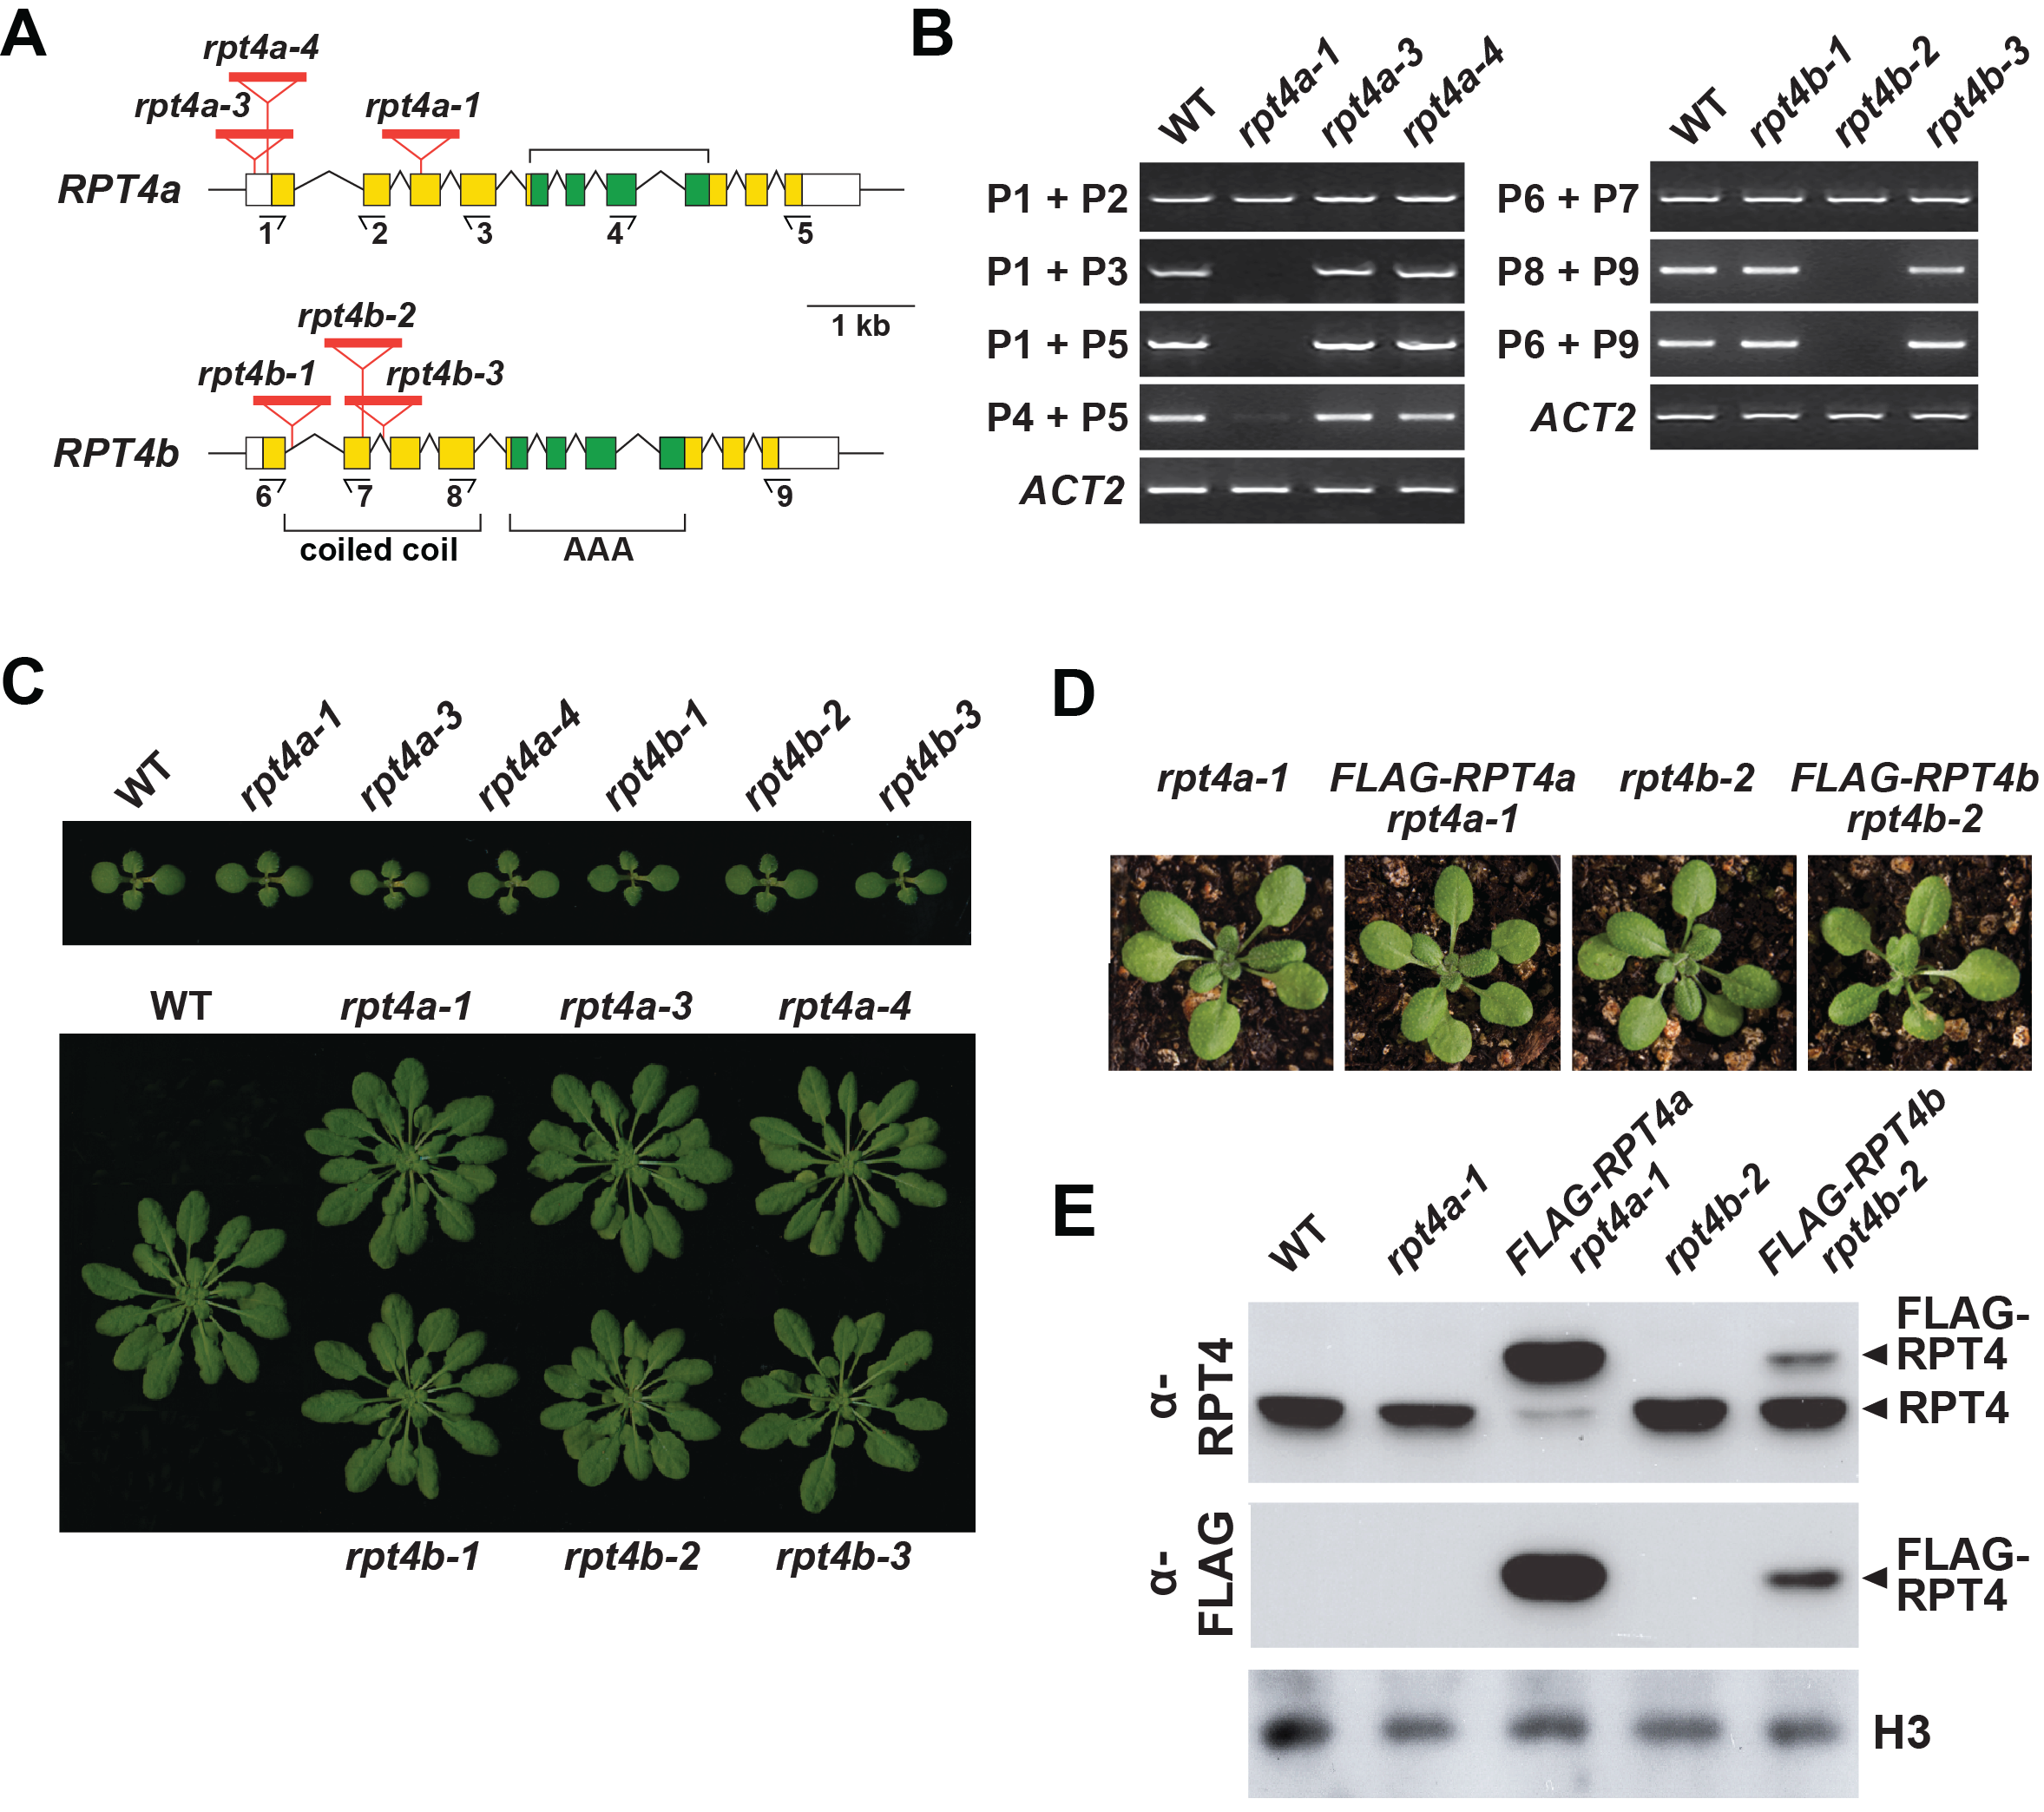
\includegraphics[width=\columnwidth]{Proteasome/rpt4abtransgenic.png}
	\mycaption{\textit{rpt4a-1} and \textit{rpt4b-2} mutants rescued with flag tagged variants}
	{\textbf{(A)} Organization of the \textit{Arabidopsis} \textit{RPT4a} and \textit{RPT4b} genes with insertion points shown for T-DNA alleles of \textit{RPT4a} and \textit{RPT4b}. \textbf{(B)} RT-PCR analysis of the \textit{RPT4a} and \textit{RPT4b} transcripts in wild type and \textit{rpt4a} and \textit{rpt4b} mutant seedlings showing aberrant \textit{RPT4a} transcripts in \textit{rpt4a-1} and abnormal \textit{RPT4b} mRNAs in \textit{rpt4b-2} plants. \textbf{(C)} Homozygous \textit{rpt4} mutants show a phenotype similar to wild-type control. The top panel shows plants grown for 10-days in a 16-hour photoperiod, while the lower panel shows plants grown for 42 days in an 8-hour photoperiod. \textbf{(D)} Replacing the wild-type \textit{RPT4a} and \textit{RPT4b} with their respective flag-tagged variants show plants with normal growth when grown for 7 days on GM plates and then grown in soil for two weeks. \textbf{(E)} Immunoblots using anti-RPT4 and anti-FLAG antibodies confirm the presence of the tag and an increased size due to the FLAG tag, which is reactive to the anti-FLAG antibody. A loading control for histone-3 is shown.}
	\label{fig:transgenic}
\end{figure}
DNA sequence analysis of the \textit{rpt4a/b} mutants determined the insertion sites to be at nucleotides 681, -278, and -24 for \textit{rpt4a-1}, \textit{rpt4a-3} and \textit{rpt4a-4} and 151, 409, and 558 for \textit{rpt4b-1}, \textit{rpt4b-2}, and \textit{rpt4b-3}, from the ATG start codon respectively. The \textit{rpt4a-1} and \textit{rpt4b-2} alleles were particularly notable because the T-DNA insertions sites disrupted the coding regions at 88 and 101 residues upstream of the AAA-ATPase cassette (Figure \ref{fig:suprpt4}) for each polypeptide which would likely block accumulation of the full length transcript (Figure \ref{fig:transgenic} B). This possibility was confirmed by RT-PCR analysis of RNA extracted from seedlings homozygous for either \textit{rpt4a-1} or \textit{rpt4b-2} showing that the plants failed to accumulate the corresponding full-length transcripts (Figure \ref{fig:transgenic} B, Primers P1 + P5, and Primers P6 + P9 respectively). However, low levels of the 5$^{\prime}$ region was amplified using primers that were 5$^{\prime}$ to the insertion site in both \textit{rpt4a-1} and \textit{rpt4b-2} plants (Primers P1 + P2, and Primers P6 + P7) suggesting that  a transcript for the 5$^{\prime}$ region still accumulates. Additionally, a small amount of product relative to wild type was also detected 3$^{\prime}$ to the insertion site for \textit{rpt4a-1} suggesting some mRNA from this region can also accumulate. At the protein level, an immunoblot analysis of SDS-PAGE-separated proteins from \textit{rpt4a-1}, \textit{rprtb-2} and wild type Col-0 seedlings showed reduction in RPT4 protein in \textit{rpt4a-1} compared to wild type, but little to no change in \textit{rpt4b-2} (Figure \ref{fig:transgenic} E). While RPT4a is the dominant isoform with 169 expressed sequence tags as compared to 39 for RPT4b \citep{berardini15}, our data detected a stronger reduction in RPT4a levels, as compared to RPT4b. There were no differences in RPT4 immunoreactivity between RPT4a and RPT4b (communications with Kwang-Hee Lee), therefore a more complex regulation of global RPT4a/b expression than anticipated may occur.  The mutants were phenotypically indistinguishable to wild-type when grown on agar plates for 10 days in a long day (LD) photoperiod (16 h light / 8 h dark) or when transferred to unfertilized soil and grown until 42 days old in a short-day photoperiod (8 h light / 16 h dark) (Figure \ref{fig:transgenic} C).  Taken together these data suggest that the two RPT4 isoforms are not essential by themselves.

Plants containing the mutant alleles \textit{rpt4a-1} and \textit{rpt4b-2} were transformed with their respective 2XFLAG-tagged genomic variants and selected for stable transgene insertion. Each construct included codons for a 2XFLAG tag and the genomic region including introns that bracketed the \textit{RPT4a/b} coding regions with expression drive by the promoter and 5$^{\prime}$ UTR regions of each locus (see Experimental Procedures). The initial transformants were self-fertilized and the homozygous lines for both the \textit{rpt4} T-DNA insertion and the transgene were identified in the Basta resistant progeny by genomic PCR.  Immunoblot analysis of proteins extracted from \textit{RPT4a/b::FLAG-RPT4a/b}-transformed plants detected accumulation of the FLAG-RPT4 proteins, which were larger than the corresponding native RPT4 polypeptides when detected with anti-RTP4 antibodies, and could be detected with anti-FLAG antibodies (Figure \ref{fig:transgenic} E).  The lower bands in the anti RPT4 immunoblot were likely RPT4b in the case of the \textit{rpt4a-1} mutant, and RPT4a in the case of the \textit{rpt4b-2} mutant. The transformed plants were phenotypically indistinguishable from wild type, implying that ectopic expression of either isoform bearing the 2X-FLAG tag was not detrimental to growth and development (Figure \ref{fig:transgenic} D).  Taken together these data showed that transgenic plants expressing their respective FLAG-tagged RPT4 variants displayed no gross morphological defects.

	Using the strategy first described by Book \textit{et al}. \citep{book10}, we exploited the homozygous \textit{FLAG-RPT4a/b rpt4a/b} seedlings to affinity purify 26S proteasomes via the RP. Briefly, frozen seedlings were homogenized in a tissue extraction buffer (see Experimental Procedures), clarified by centrifugation, and subjected to anti-FLAG chromatography, using FLAG peptide for gentle elution.  To enrich for the 26S particle, 20 mM ATP was included in the indicated buffers to stabilize the CP/RP association \citep{book10, liu06}. To enrich for just the RP (using FLAG-RPT4a/b) or the CP (using PAG1-FLAG) the same protocol was used except that ATP was omitted from the buffers. As a control, we also attempted to purify 26S proteasomes from wild-type tissues.  Under conditions where 20 mM ATP was included in the purification buffer (indicated with a + in Figure \ref{fig:purification} A), the FLAG-RPT4a/b affinity purified samples showed a comparable protein banding pattern after SDS-PAGE as compared to the PAG1-FLAG affinity-purified samples suggesting a similar complement of proteins were present (Figure  \ref{fig:purification} A). The only notable exception was the observation of a band that likely represented the FLAG-tagged PAG1 subunit (indicated with a black arrow) in the PAG1-FLAG samples \citep{book10}. The size-shifted RPT4 subunits seemed to be masked by other subunits and were not readily identifiable via silver staining alone. Importantly, the mock affinity-purified samples from wild-type tissue showed very few contaminating proteins as judged by protein staining with silver, which was important for down-stream tandem mass-spectrometry (MS/MS) analyses. Overall, these affinity purification strategies based on either RPT4a or RPT4b successfully purified 26S proteasomes from whole \textit{Arabidopsis} seedlings.
 \begin{figure}[p]
	\centering
	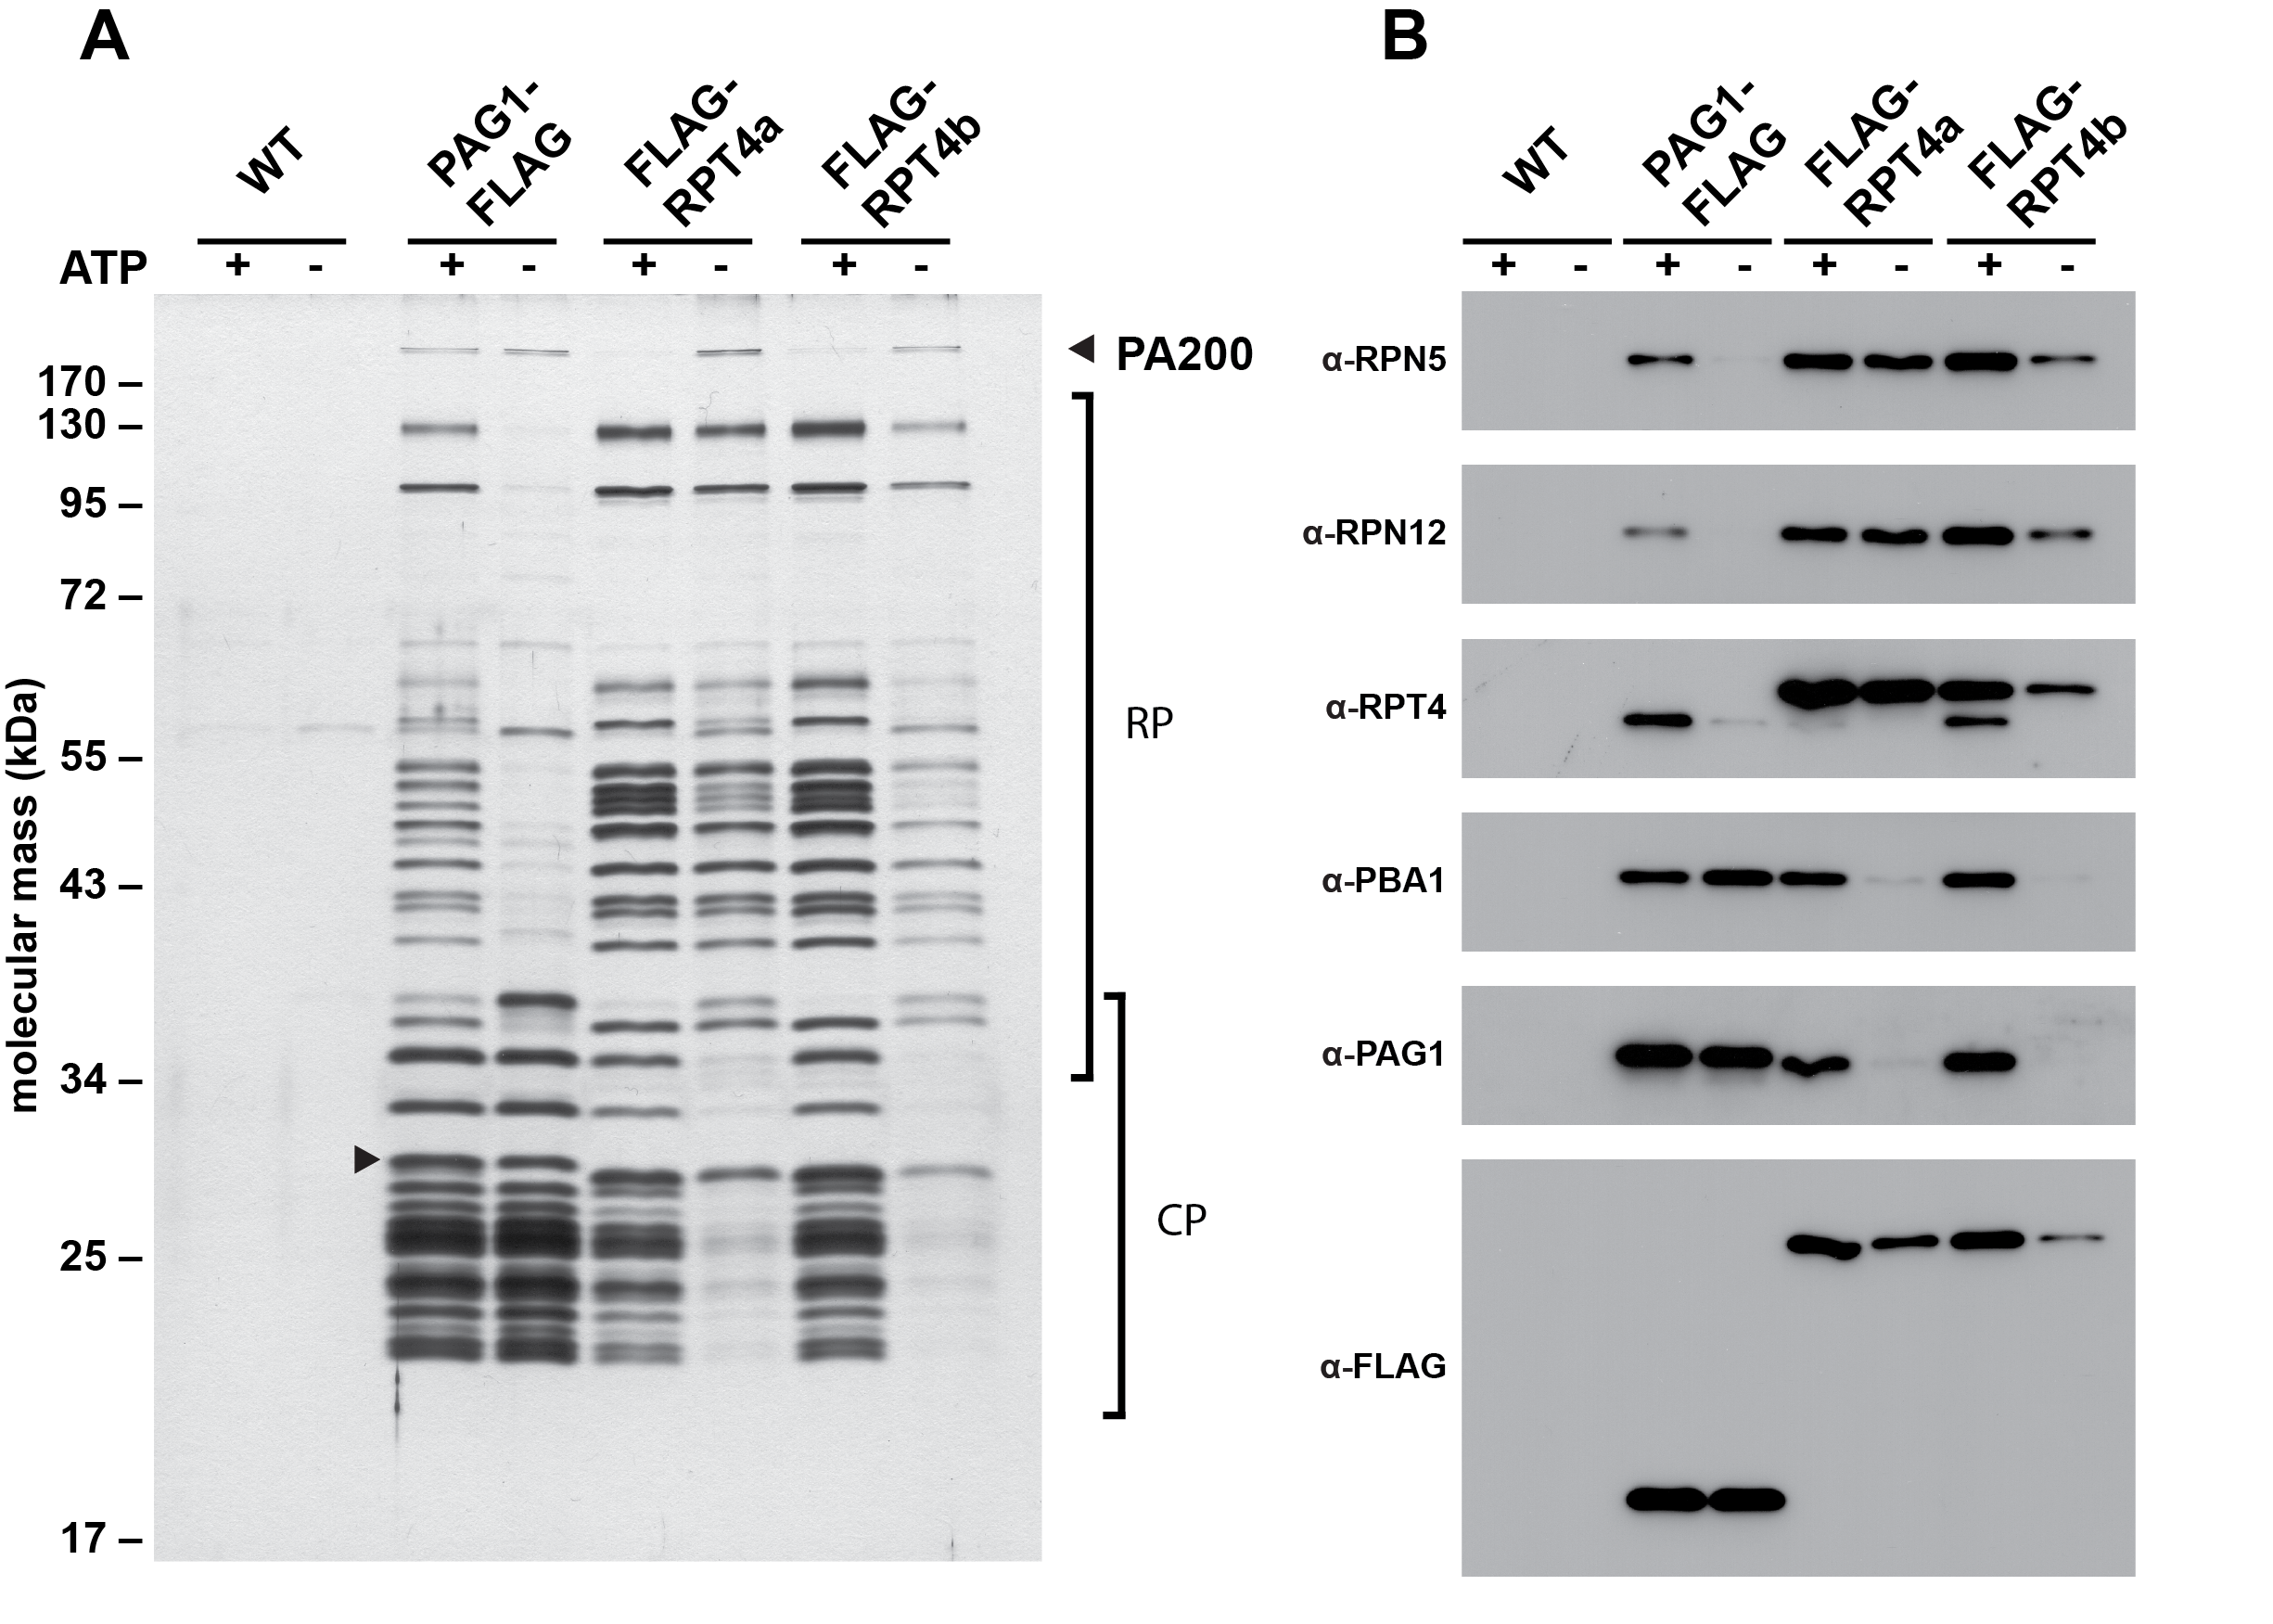
\includegraphics[width=\columnwidth]{Proteasome/purification.png}
	\mycaption{Protein composition of affinity-purified proteasomes from FLAG-RPT4a-, FLAG-RPT4b-, and PAG1-FLAG-expressing plants and from mock wild-type controls in the presence (+) or absence (-) of 20mM ATP.}
	{\textbf{(A)} Silver stained gel of each preparation shows clear enrichment over the negative control (Col-0) with minimal contaminants, both in the presence and absence of ATP during purification. Omitting ATP from the preparations for the CP-based PAG1-FLAG pulldown shows a decreased amount of RP subunits, while both RP-based subunit pulldowns show a decrease in the amount of CP subunits. \textbf{(B)} Immunoblots for various proteasome subunits for both the RP and the CP show a clear enrichment of proteasome subunits as compared to the wild type mock affinity purification control.  As shown in the silver stain, omitting ATP from the preparations in each affinity purification causes a decrease in association of the alternative sub-particle (decrease in RP for CP pulldowns, and decrease in CP for RP pulldowns).}
	\label{fig:purification}
\end{figure}	
	When ATP was omitted from the purification buffer, there was clear enrichment for the CP in PAG1-FLAG samples, and clear enrichment for the RP in both the FLAG-RPT4a and FLAG-RPT4b samples, as judged by the size and intensity of the protein bands in Figure \ref{fig:purification} A. Immunoblot analysis of these samples showed clear enrichment for two CP subunits PAG1 and PBA1 in the CP-based samples affinity-purified in the absence of ATP, as compared to the RP subunits RPT4, RPN5, and RPN12 (Figure \ref{fig:purification} B). There was also clear enrichment for the three RP subunits in the RP-based affinity purified samples when ATP was omitted from the purification as compared to the CP subunits that were immunoblotted.  Taken together, these data show that 26S proteasomes can be easily purified based on a RP affinity tag, and that both isoforms for a single subunit will work. By omitting ATP from the buffer, we were able to enrich for subunits of the CP or the RP utilizing affinity purifications from PAG1-FLAG and FLAG-RPT4a/b expressing tissues, respectively. 

\subsection{MS/MS Analyses of RPT4a/b Affinity-Purified Proteins Identifies a Similar Complement of Proteins as PAG1-FLAG Affinity Purifications}
	Previous MS/MS analyses of affinity preparations based on PAG1-FLAG identified the fundamental subunits that make up the 26S proteasome, including the CP $\alpha$-subunits (PAA-PAG), the CP $\beta$-subunits (PBA-PBG), the RP AAA-ATPases (RPT) (RPT1-6), and the RP non-ATPase subunits (RPN) (RPN1-3 and RPN5-12). Most subunits are encoded as a paralogous gene pair (named 1 and 2 for CP subunits, and a and b for RP subunits) and most isoforms were found to be incorporated in the complex \citep{book10}. We wanted to verify that our affinity purifications based on RPT4a and RPT4b also contained a similar set of proteins as in Book \textit{et al}. \citep{book10}. To do this we used label-free quantitative tandem mass spectrometry (LFQ-MS/MS) to analyze samples obtained from affinity purifications for FLAG-RPT4a, FLAG-RPT4b, PAG1-FLAG, and a mock wild-type control, in the presence and absence of ATP resulting in MaxLFQ values \citep{cox14} for each protein analyzed. Importantly, we identified all subunit isoforms previously identified by Book \textit{et al}. \citep{book10} showing that our purifications were comparable (Figure \ref{fig:MSCP}, CP $\alpha$-ring, CP $\beta$-ring, RPT, and RPN plots).  Additionally, we identified a suite of key accessory proteins found to be statistically enriched as compared to control at a false discovery rate (FDR) of 0.01 for both the CP and RP (Figure \ref{fig:MSCP} Associated Proteins).

\begin{sidewaysfigure}[p]
	\centering
	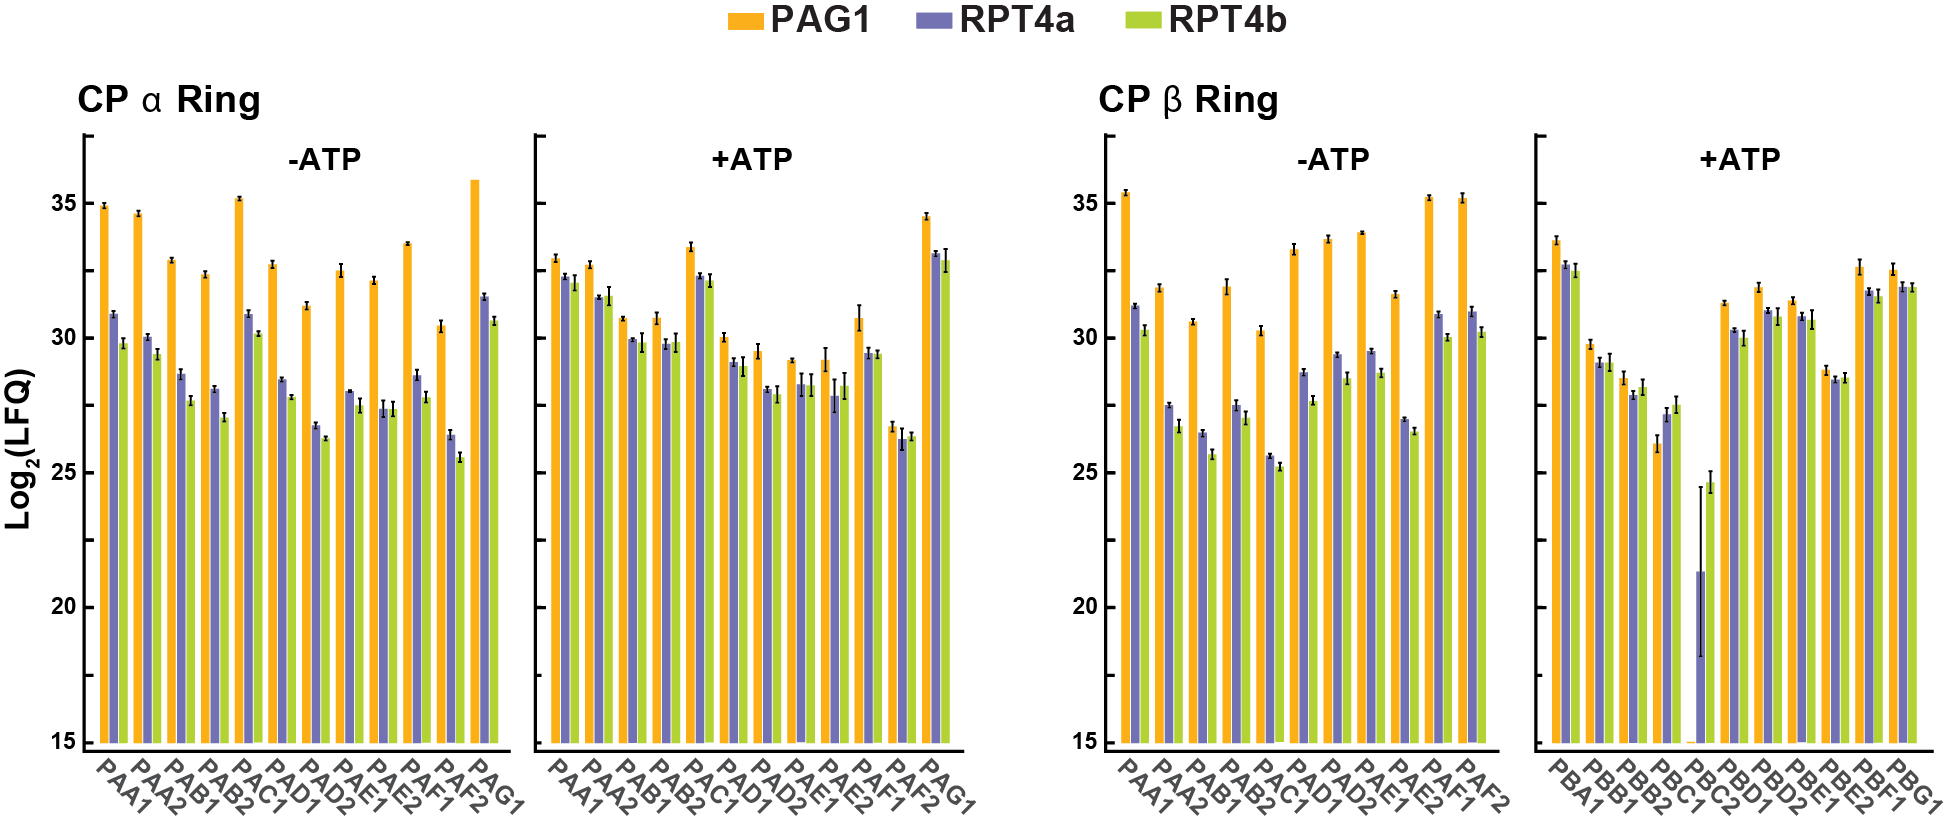
\includegraphics[width=\columnwidth]{Proteasome/MSCP.png}
	\mycaption{Label-free quantitative MS/MS analysis of affinity-purified proteins in the presence (+) or absence (-) of ATP}
	{\textbf{(CP Alpha Ring)} $\alpha$-subunits are enriched in samples that were affinity purified via the CP subunit PAG1-FLAG. This enrichment increases even further when ATP is omitted from the preparations as shown on the left side of the graph. \textbf{(CP Beta Ring)} $\beta$-subunits are enriched at a higher level when purified via the CP subunit PAG1-FLAG. This enrichment increases even further when ATP is omitted from the preparations as shown on the left side of the graph.}
	\label{fig:MSCP}
\end{sidewaysfigure}

\begin{sidewaysfigure}[p]
	\ContinuedFloat
	\centering
	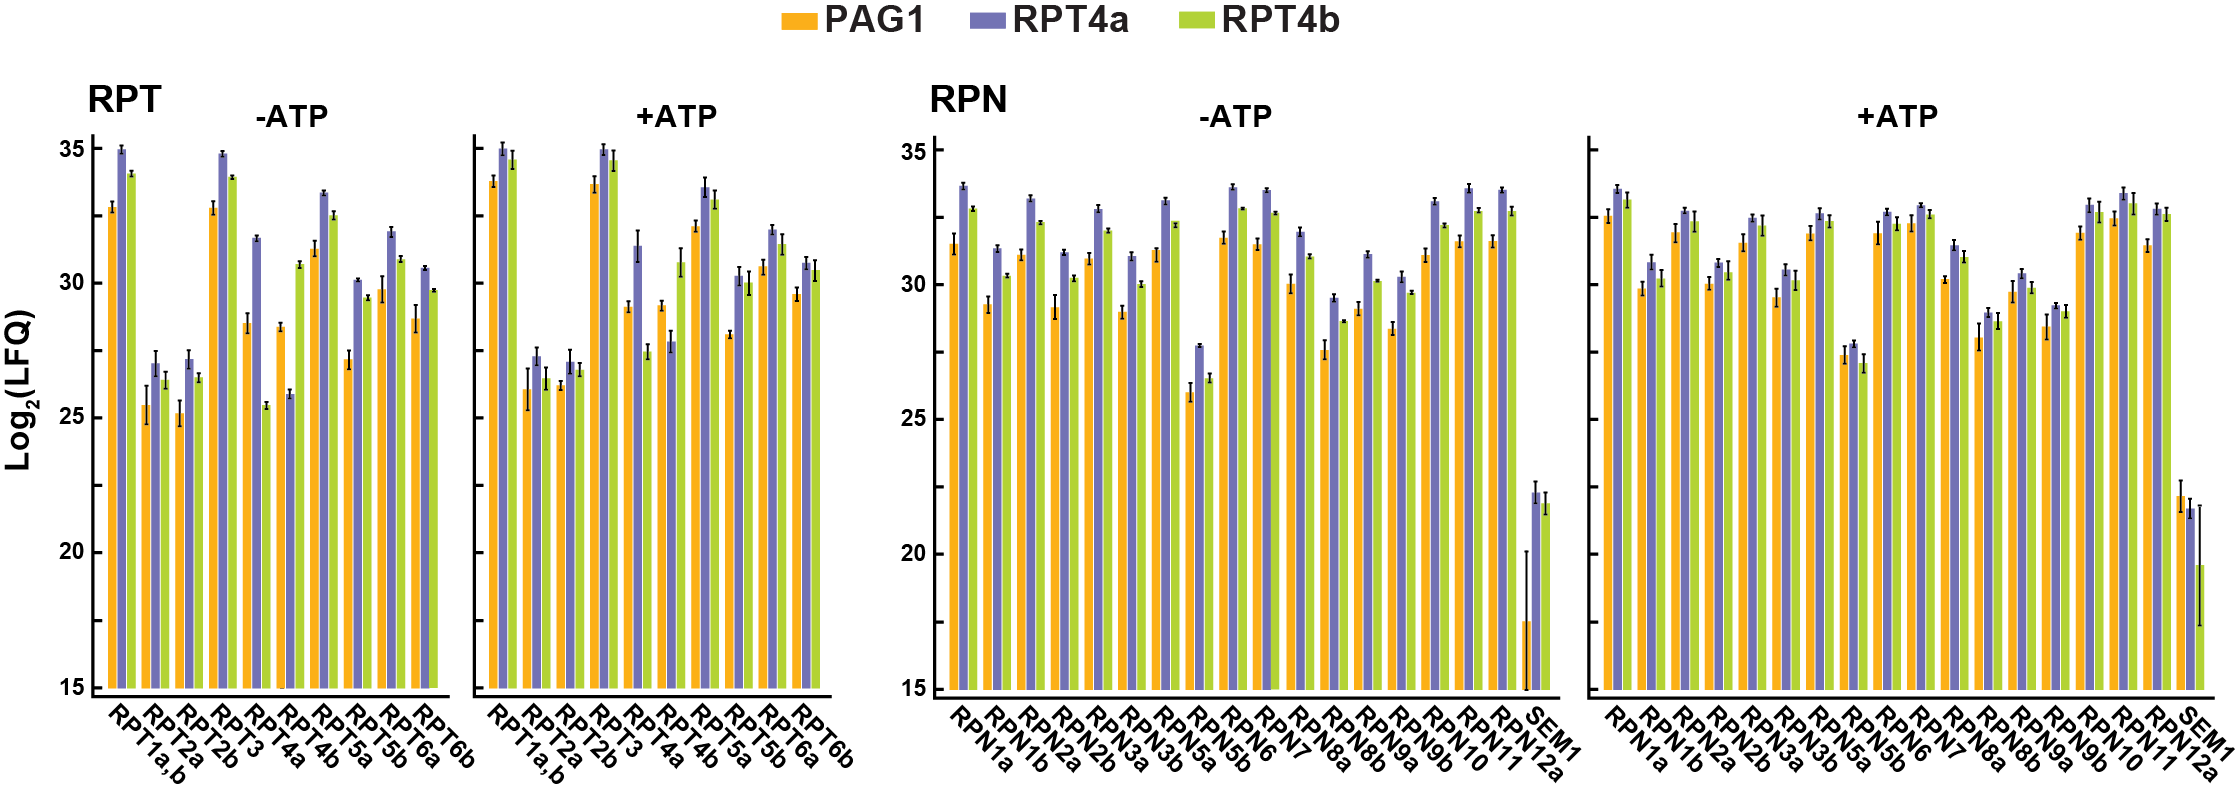
\includegraphics[width=\columnwidth]{Proteasome/MSRP.png}
	\mycaption{Label-free quantitative MS/MS analysis of affinity-purified proteins in the presence (+) or absence (-) of ATP}
	{\textbf{(RPT Subunits)} RPT subunits are enriched at a higher level when purified via RP subunits RPT4a or RPT4b. There are clear increases in the level of enrichment of the RPT4a subunit for the RPT4a affinity purifications, and clear increases in enrichment of the RPT4b subunit for the RPT4b affinity purifications. These respective increases are greater than the isoform unbiased PAG1 pulldowns. The respective enrichments of each isoform also increases when ATP is omitted, due to a decrease in the possibility of binding the alternative subunit isoform under ATP limiting conditions. \textbf{(RPN Subunits)} RPN subunits are enriched at a higher level when purified via RP subunits RPT4a and RPT4b. This enrichment increases even further when ATP is omitted from the preparations as shown on the left side of the graph.}
	\label{fig:MSRP}
\end{sidewaysfigure}

\begin{sidewaysfigure}[p]
	\ContinuedFloat
	\scalebox{.6}{
	\centering
	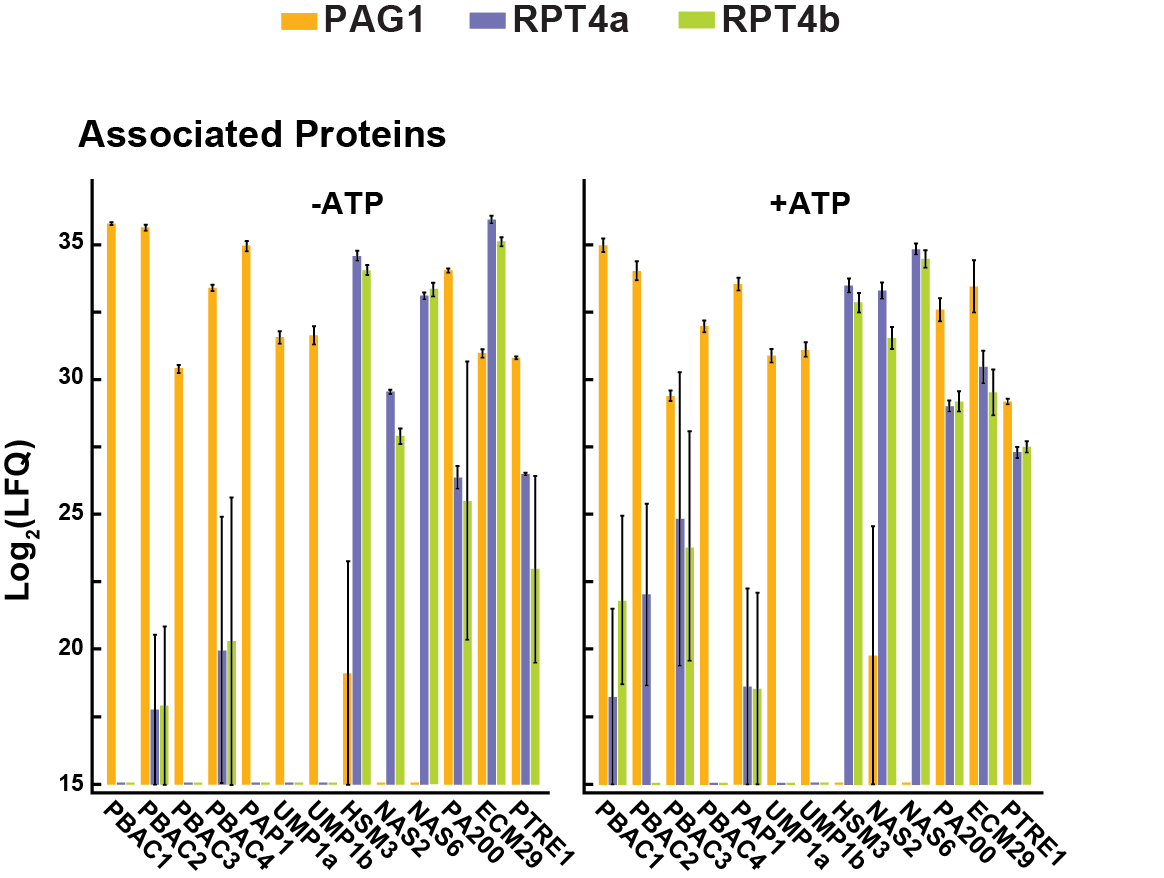
\includegraphics[width=\columnwidth]{Proteasome/MSAssociated.png}}
	\mycaption{Label-free quantitative MS/MS analysis of affinity-purified proteins in the presence (+) or absence (-) of ATP}
	{\textbf{(Associated Proteins)} Key proteins identified as proteasome interacting proteins are specifically enriched in pulldowns based on the CP subunit PAG1, and others are specifically enriched for pulldowns based on either RP subunits RPT4a or RPT4b. Please refer to Figure 4 for statistical analyses of CP and RP distributions in affinity-purified samples, and for statistical analyses that identify candidates as associated proteins.}
	\label{fig:MSAssociated}
\end{sidewaysfigure}

The CP $\alpha$- and $\beta$-subunits show higher MaxLFQ values in the PAG1-FLAG samples as compared to either FLAG-RPT4a/b sample under both plus and minus ATP conditions (Figure \ref{fig:MSCP}, CP $\alpha$-ring, CP $\beta$-ring). This suggests some free CP was purified even in the presence of ATP, and that the complexes purified were not exclusively RP-CP proteasomes. In the PAG1-FLAG samples, the CP $\alpha$ and $\beta$-subunits showed higher MaxLFQ values when ATP was omitted from the affinity purification buffer as compared to when ATP was present (Figure \ref{fig:MSCP}, CP CP $\alpha$-ring, CP $\beta$-ring). This increase is consistent with the preferential purification of the CP over the RP in the absence of ATP when using the PAG1-FLAG epitope tag.

Likewise, both affinity purifications that target the RP through FLAG-RPT4a/b, had higher MaxLFQ values for RP subunits as compared to the CP-based PAG1-FLAG samples under both plus and minus ATP conditions. When ATP was omitted from the purification, the FLAG-RPT4a/b samples had increased MaxLFQ values for RP subunits as compared to when ATP was included; however, this increase was considerably less than that observed for the CP subunits in the PAG1-FLAG samples (Figure \ref{fig:MSCP}, RPT, and RPN plots). FLAG-RPT4a samples had higher MaxLFQ values for RPT4a when compared to FLAG-RPT4b and PAG1-FLAG (Figure \ref{fig:MSCP}, RPT plot). Conversely, FLAG-RPT4b samples had higher MaxLFQ values for RPT4b when compared to FLAG-RPT4a and PAG1-FLAG (Figure \ref{fig:MSCP}, RPT plot). These data suggest that, as expected, RPT4a was enriched in the FLAG-RPT4a samples, and that RPT4b was enriched in the FLAG-RPT4b samples.

\subsection{Statistical Analysis of Affinity Enrichments for FLAG-RPT4a Show Little to No Difference When Compared to FLAG-RPT4b}
While mammals and yeast can form only a few types of proteasomes, \textit{Arabidopsis}, with its many subunit paralogs, can potentially form a much wider array of proteasome isotypes. By comparing samples enriched for RPT4a and RPT4b using a Significant Analysis of Microarray (SAM) test at 0.01 FDR, we determined if any additional subunit isoforms (or other associated proteins) are incorporated preferentially, which would suggest that \textit{Arabidopsis} can form proteasome isotypes. Surprisingly, this statistical analysis revealed that only when ATP was omitted from the purifications were the samples statistically enriched for either RPT4a or RPT4b, respectively (Figure \ref{fig:suprpt4avsrpt4b} B). While RPT4 and RPT4b were enriched in the samples in which ATP was included in the purification, they were not statistically significant by the SAM test at 0.01 FDR (Figure \ref{fig:suprpt4avsrpt4b} A). Additionally, the 26S proteasome subunits have larger MaxLFQ values in the FLAG-RPT4a sample suggesting a slightly more efficient purification for the proteasome with the RPT4a isoform. Furthermore, no significant enrichment of any other subunit isoforms was observed. As such these data suggest that there are no major differences in protein composition between affinity purifications for FLAG-RPT4a or FLAG-RPT4b other than statistically enriching for each individual isoform when ATP was omitted from the purification. This indicates that plants may assemble their proteasome randomly with respect to isoform incorporation under the conditions tested. 

\subsection{Statistical Analyses of LFQ-MS/MS Data Show Affinity Preparations Targeting Either the CP or RP Specifically Enrich for Their Respective Subcomplexes}
The LFQ-MS/MS data allowed us to perform a more formal statistical test for the enrichment of the RP over the CP in samples affinity purified from the RP subunits FLAG-RPT4a/b, and for the enrichment of the CP over the RP in samples affinity purified from CP subunit PAG1-FLAG. We estimated the distribution of RP and CP subunits in these samples using kernel density estimations (KDE) of MaxLFQ values as compared to our wild-type mock-affinity purifications as a negative control (Figure \ref{fig:volcanos} below each volcano plot, and larger plots in Figure S3).  As the KDE distributions were not normal, two non-parametric statistical tests, Kolmogorov-Smirnov (KS) and median test, were used to determine if there was specific enrichment of particular proteasome sub-complexes (RP vs CP) from the different affinity purifications. The KS test determines if the two distributions are different in shape or position, and the median test determines if the distribution’s medians are statistically different.

\begin{sidewaysfigure}[p]
	\centering
	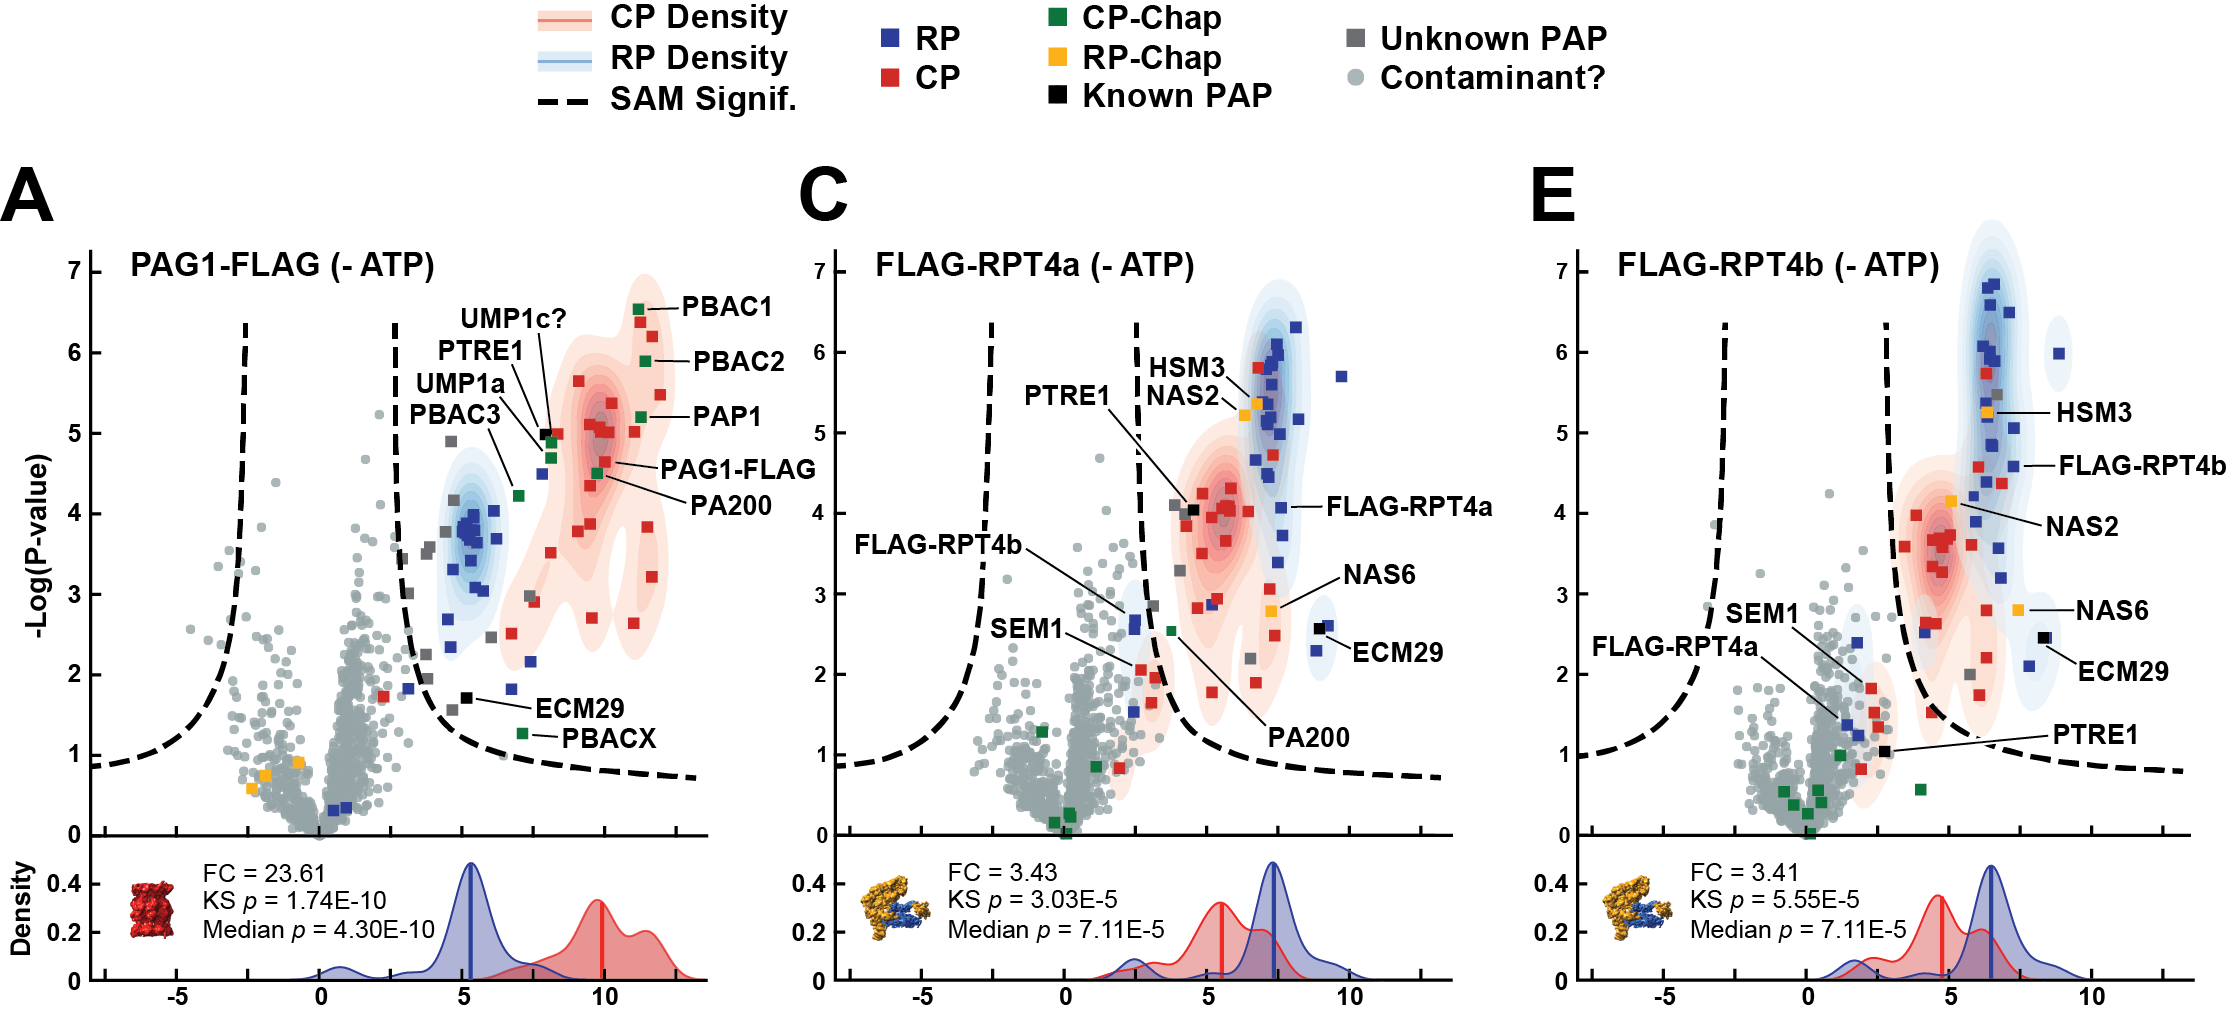
\includegraphics[width=\columnwidth]{Proteasome/Volcanosplit1.png}
	\mycaption{Volcano Plots comparing proteasome affinity purifications under both plus and minus ATP conditions relative to WT controls, allow identification of statistically significant interacting partners for the proteasome}
	{Volcano plots comparing affinity purifications for PAG1-FLAG \textbf{(A and B)}, FLAG-RPT4a \textbf{(C and D)}, and FLAG-RPT4b \textbf{(E and F)} against their respective WT mock affinity purification control are shown. The top panels \textbf{(A, C, and E)} show comparisons for samples purified in the absence of ATP, while the lower panels \textbf{(B, D, and F)} show comparisons for samples purified in the presence of ATP. Two-dimensional Kernel Density Estimations (KDE) are shown for CP subunits in red and RP subunits in blue. Larger KDE plots are available in Figure S3. CP subunits are labeled as red squares, while RP subunits are labeled as blue squares. Proteins outside the dashed lines are statistically significantly differentially represented in purified samples relative to control as judged by a significant analysis of microarray or (SAM) test at 0.01 false discovery rate. Proteins likely involved in CP assembly are shown as green squares, while proteins likely involved in RP assembly are shown as yellow squares. Known proteasome associated proteins or PAPs are labeled as black squares, while unknown PAPs are labeled in grey squares. Proteins identified that did not reach SAM significance are labeled as grey circles.}
	\label{fig:volcanos1}
\end{sidewaysfigure}

\begin{sidewaysfigure}[p]
	\ContinuedFloat
	\centering
	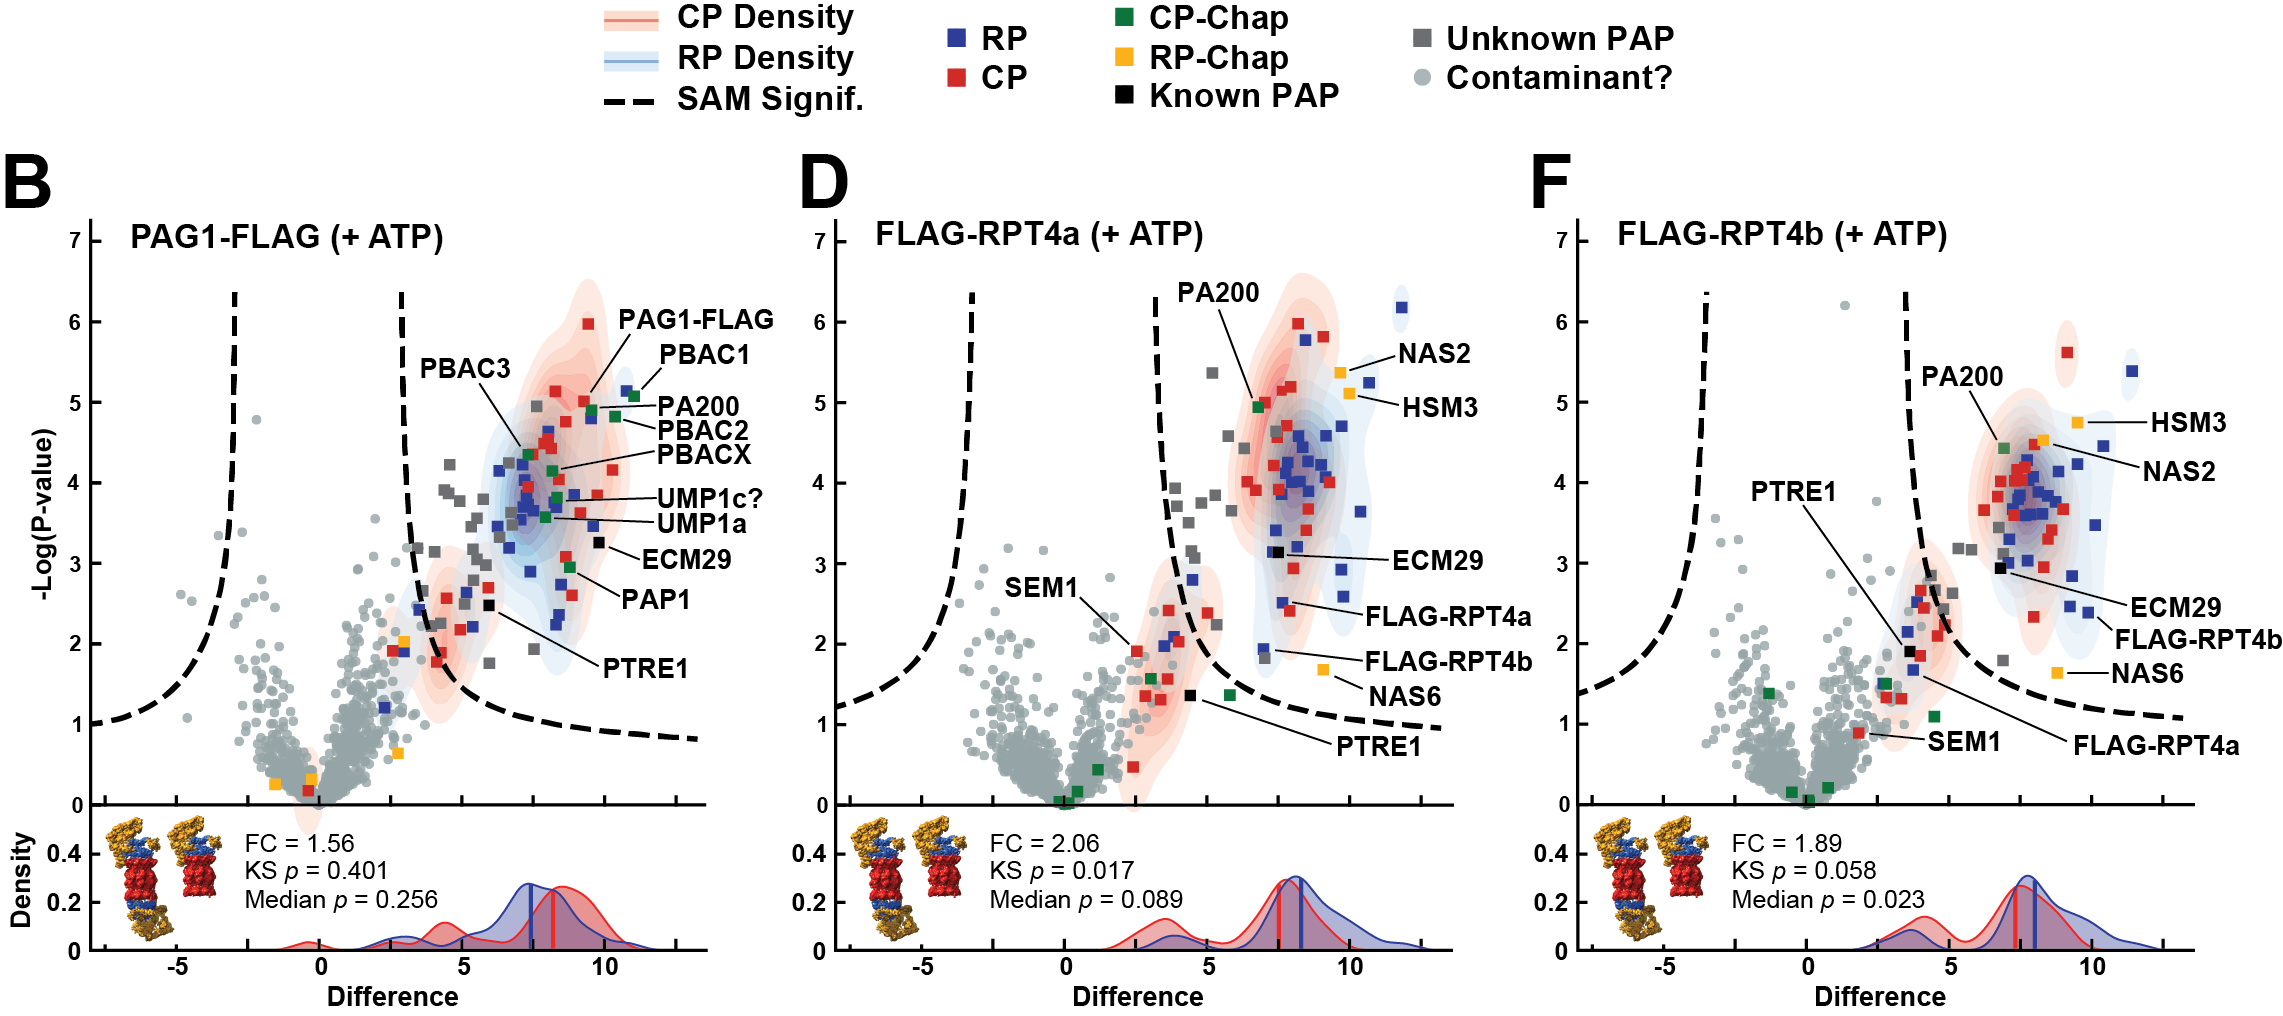
\includegraphics[width=\columnwidth]{Proteasome/Volcanosplit2.png}
	\mycaption{Volcano Plots comparing proteasome affinity purifications under both plus and minus ATP conditions relative to WT controls, allow identification of statistically significant interacting partners for the proteasome}
	{Volcano plots comparing affinity purifications for PAG1-FLAG \textbf{(A and B)}, FLAG-RPT4a \textbf{(C and D)}, and FLAG-RPT4b \textbf{(E and F)} against their respective WT mock affinity purification control are shown. The top panels \textbf{(A, C, and E)} show comparisons for samples purified in the absence of ATP, while the lower panels \textbf{(B, D, and F)} show comparisons for samples purified in the presence of ATP. Two-dimensional Kernel Density Estimations (KDE) are shown for CP subunits in red and RP subunits in blue. Larger KDE plots are available in Figure S3. CP subunits are labeled as red squares, while RP subunits are labeled as blue squares. Proteins outside the dashed lines are statistically significantly differentially represented in purified samples relative to control as judged by a significant analysis of microarray or (SAM) test at 0.01 false discovery rate. Proteins likely involved in CP assembly are shown as green squares, while proteins likely involved in RP assembly are shown as yellow squares. Known proteasome associated proteins or PAPs are labeled as black squares, while unknown PAPs are labeled in grey squares. Proteins identified that did not reach SAM significance are labeled as grey circles.}
	\label{fig:volcanos2}
\end{sidewaysfigure}

The KDE distribution for the CP as compared to the RP from samples affinity purified in the absence of ATP using PAG1-FLAG showed both the KS and the median \textit{p}-values being much less than 0.01, at 1.74E-10 and 4.3E-10, respectively (Figure 4 and S3 A). This suggests that the distributions are different, and that their medians were different with a greater than 20 fold increase in CP over RP. Conversely the KDE distributions for the samples affinity purified in the presence of ATP using PAG1-FLAG (Figure 4 and S3 B) overlap to a higher degree, with both the KS and Median \textit{p}-values > 0.01 at 0.401 and 0.256, respectively. This indicates that in samples affinity purified in the presence of ATP that the RP and CP distributions were not significantly different, and that their means were similar. Although not statistically significant, a 1.5 median fold change was observed for the CP over the RP in samples affinity purified in the presence of ATP using PAG1-FLAG suggesting that there may be some CP enriched as compared to the RP. These statistical analyses showed that, as expected, we were able to successfully enrich for the CP over the RP when affinity purifying from PAG1-FLAG expressing tissue.

	Conversely, in samples using the RP-based FLAG-RPT4a/b purified in the absence of ATP, the KDE distributions showed enrichment for the RP over the CP, with a fold change of 3.43 and 3.41 for the RPT4a and RPT4b subunits respectively (Figures 4 and Figures S3 C and E, respectively). Both the KS (3.303E-5 for RPT4a and 5.55E-5 for RPT4b) and median \textit{p}-values (7.11E5 for RPT4a and 7.11E-5 for RPT4b) were < 0.01, suggesting that the two distributions were statistically different and had different medians. Again, contrasting this with the samples purified in the presence of ATP using FLAG-RPT4a and FLAG-RPT4b (Figures 4 and Figures S3 D and F, respectively), the KDE distributions overlap with both the KS (0.017 for RPT4a and 0.058 for RPT4b) and median \textit{p}-values (0.089 for RPT4a and 0.023 for RPT4b) were > 0.01, suggesting that the RP and CP distributions are similar. Although not statistically significant, we still observed a two-fold-change enrichment in both FLAG-RPT4a/b samples purified in the presence of ATP for the RP over the CP. In summary, these KDE distributions and statistical analyses provide further support for enrichment of either the CP or the RP, as expected, when samples were affinity purified in the absence of ATP via PAG1-FLAG, or FLAG-RPT4a/b, respectively.

\subsection{Statistical Analysis of Affinity Purifications Enriched for the RP or CP Identifies Proteasome-Associated Proteins and Putative Assembly Chaperones Specific to Each Subcomplex}
	The ability to affinity-enrich both the CP and the RP from \textit{Arabidopsis} under gentle non-denaturing conditions without the need for high salt washes may enable identification of associated proteins, particularly those which may be more loosely bound. Additionally, targeting the RP or CP enables the identification of proteins that may be associating with either or both subcomplexes specifically. The previous data represented in Figure 3 showed the raw MaxLFQ values for some of the relevant associated proteins; however, a formal statistical test against mock affinity purifications was important given the high number of proteins identified and quantified via LFQ-MS/MS. To better understand the suite of proteins that are statistically enriched in samples that target the CP or RP specifically we compared the LFQ-MS/MS data obtained from our affinity purifications against their respective wild-type controls using volcano plots and SAM tests at 0.01 FDR.
	
Affinity purifications enriching for the CP via PAG1-FLAG, performed either in the presence or absence of ATP (Figure 4A and 4B respectively) show statistical enrichment for two orthologs of the UMP1 CP assembly chaperone, UMP1a and UMP1b. The \textit{Arabidopsis} genome encodes a third \textit{UMP1} ortholog, \textit{UMP1c}; however, we have no experimental evidence that UMP1c associates with the proteasome, even though it has several tryptic peptides from an extended C-terminal domain that could differentiate it from UMP1a/b (Figure S4). UMP1a, and UMP1b are considerably higher expressed at 90 and 55 ESTs as compared to UMP1c which had only 7 ESTs \citep{berardini15}, suggesting that UMP1c may be lowly expressed, or possibly a pseudogene. 

Intriguingly, these samples also show statistical enrichment for a suite of putative CP assembly chaperones (Proteasome Biogenesis Associated Chaperone) PBAC1-4 (Figure 4A and 4B). Although their annotation in The \textit{Arabidopsis} Information Resource v10 (TAIR10) was incomplete, an InterProScan of their respective sequences supported these identifications (Table S3A). While PBAC1 was annotated as having a PBAC2 domain, the expectation value of 3.4E-6 was much lower than the expectation value of 1E-29 for the PBAC2 domains in the potential PBAC2 homologue. Additionally, PBAC1 and PBAC2 were previously identified by iterative PSI-BLAST with the human PAC1 and PAC2 orthologs in two separate studies \citep{kusmierczyk11, le07} which aids in our assignment of PBAC1 and PBAC2. This PSI-BLAST based analysis was repeated using human PAC1-4, which identified PBAC1-4 as the top hits for these proteins in \textit{Arabidopsis} (Table S3B). Protein sequence alignments for PBAC1-4 show that these proteins are conserved across plants but that they show little conservation with orthologs outside the plant kingdom with < 15\% protein sequence identity (Figure S5-S8).  All statistically significant interactors from PAG1-FLAG affinity purifications performed in both the presence or absence of ATP are available in Table S4.

As shown in Figure 4 C-F, UMP1a/b and PBAC1-4 were not significantly enriched in our affinity purifications targeting the RP, suggesting that these proteins interact with the CP specifically. However, affinity purifications that targeted the RP through either FLAG-RPT4a or FLAG-RPT4b showed statistically significant enrichment over controls for the putative orthologs of RP assembly chaperones HSM3, NAS2, and NAS6 (Figure 4 C-F). Importantly, these putative RP assembly chaperones were also absent from our affinity purifications that targeted the CP, suggesting that these proteins are RP specific interactors. All statistically significant interactors from FLAG-RPT4a and FLAG-RPT4b affinity purified in the presence or absence of ATP are available in Table S5 and Table S6. Several accessory proteins are common to both CP and RP purifications including the alternate capping particle PA200 \citep{book10}, ECM29 that is involved in stabilizing the CP-RP association \citep{lehmann10}, and the recently identified proteasome inhibitor 31 related protein PTRE1, which is involved in modulating proteasome activity in response to auxin \citep{yang16}. 

\subsection{A Novel Plant Proteasome-Associated Protein, PAP1, Interacts with a Putative CP Assembly Chaperone}
An intriguing plant-specific protein, named here Proteasome Associated Protein 1 or PAP1 was identified and significantly enriched in affinity preparations that targeted the CP (Figure 4). While PAP1 had no domains of known function, as determined by InterProScan (Table S3A), it did contain a C-terminal HbYX (hydrophobic amino acid, followed by a tyrosine, followed by any amino acid) motif. This HbYX motif is commonly found in proteins that intercalate between the $\alpha$-rings of the CP \citep{kusmierczyk11}. This motif is found in both the plant specific PAP1, and in the assembly chaperone PBAC1 (Figure 5A) as well as the conserved yeast assembly chaperones Pba1 and Pba2 \citep{kusmierczyk11}. However, Pba2/PBAC2 orthologs outside of yeast typically contain a C-terminal HbF motif, with the only notable exception being the moss \textit{Physcomitrella patens} which instead contains a HbYX motif.   To confirm whether PAP1 did indeed interact with the proteasome, we generated transgenic plants expressing HA-tagged PAP1 in the \textit{PAG1::PAG1-FLAG pag1-1} background. Figure 5B shows immunoblots of SDS-PAGE separated samples from an affinity purification of HA-PAP1 utilizing anti-HA beads. HA-PAP1 expressed at very low levels in transgenic plants (Figure 5B, input). However, upon immunopurification and detection with anti-HA antibodies we were able to detect HA-PAP1, the FLAG-tagged CP $\alpha$-subunit PAG1, and the FLAG-less PAG1 product that likely resulted from cleavage of the FLAG tag during overnight incubation \citep{book10}. Low levels of both the CP $\beta$-subunit PBA1, and RPN1 subunit were also detected in these samples. 

To identify which putative \textit{Arabidopsis} assembly chaperones might interact, we performed a yeast two-hybrid (Y2H) interaction assay for all pairwise combinations of PBAC1-4, and PAP1 (Figure 5C). We hypothesized that PAP1 may be a CP assembly chaperone and that it may interact with one or more of the other putative assembly chaperones. The Y2H showed pairwise interaction for PBAC1 and PBAC2, and pairwise interaction for PBAC3 and PBAC4 regardless of whether they were attached to the GAL4 activating or binding domains (Figure 5C). These interactions were consistent with how the CP assembly orthologs in other organisms interact \citep{murata09}.  Taken together these data suggested these proteins might form heterodimeric pairs, like other CP assembly chaperone orthologs. Importantly, we saw no interaction from PBAC1 or PBAC2 to PBAC3 or PBAC4 pairs in this Y2H, suggesting these putative assembly chaperones form separate complexes like their orthologs in mammals and yeast. Interestingly, we observed PAP1 interacting with PBAC1, which suggested that it may be part of the plant assembly chaperone PBAC1/2 complex (Figure 5C). 

Because these interactions were analyzed in yeast, which contain their own assembly chaperones that might interfere with interactions between plant subunits, we wanted to verify that PAP1 interacted with PBAC1 \textit{in planta}. To do this we tested several pairwise interactions by bimolecular fluorescent complementation (BiFC) via transient expression in \textit{Nicotiana benthamiana} leaves. Figure 5D shows confocal images of transiently expressed PAP1, PBAC1, PBAC2, and PBAC3 with either the N- or C-terminal half of YFP (NYFP and CYFP respectively) attached as a translational fusion to the N-terminus of each putative assembly chaperone. As controls, PAP1 and PBAC1-3 were tested for auto-activation against NYFP or CYFP alone with no strong auto-activation being observed (Figure S10B). We again observed interactions between PBAC1 and PBAC2, regardless of their attachment to the N or C terminal halves of YFP based on their strong fluorescent intensity (Figure 5D). Additionally, we saw an interaction between PAP1 and PBAC1, showing that PAP1 can interact with PBAC1 \textit{in planta}.  Consistent with our Y2H data, there was no evidence of strong interaction between PAP1 and PBAC3 (Figure 5D). 

\subsection{Inhibition of the Proteasome Results in Formation of Distinct Proteasome Sub-Species Containing Putative CP Assembly Chaperones}
Upon inhibition with the proteasomal inhibitor MG132, most proteasome genes are coordinately upregulated by a pair of NAC transcription factors, NAC53 and NAC78, as the plants attempt to synthesize more proteasomes in an effort to increase degradation capacity \citep{gladman16}. Additionally, after prolonged inhibition the complex becomes heavily ubiquitylated and is turned over via autophagy, likely as a clearing mechanism for inhibited complexes \citep{marshall15}. We reasoned that treatment with MG132 might lead to an increase in the population of newly assembling proteasomes, potentially allowing us to observe proteasome assembly intermediates. As such, proteasomes were purified in the presence of ATP from \textit{PAG1::PAG1-FLAG pag1-1} tissue treated for 16 hours with or without MG132. A silver stain of SDS-PAGE-separated proteins affinity-purified from MG132-treated tissue showed successful purification of the 26S proteasome under these conditions (Figure 6A) with the only notable difference in the treated sample being an increased association of PA200, which was also observed by Book et al. \citep{book10}. An anti-ubiquitin immunoblot of the same samples (Figure 6B), showed extensive ubiquitylation of the particle consistent with data observed by Marshall et al \citep{marshall15}.

Non-denaturing native-PAGE of affinity-purified proteasomes were performed to determine if any novel complexes could be observed. Intriguingly, silver staining of samples affinity-purified from MG132-treated tissue revealed a smear below the canonical CP band (Figure 6B). Additionally, extra bands were observed above the canonical CP band, which may represent stalled intermediates with the alternate capping particle PA200 \citep{li07}. To identify the proteins contained in the bands shown in Figure 7B, we cut the corresponding gel slices, trypsin-digested the proteins, and then analyzed the resulting peptides via MS/MS. A LFQ-MS approach was used to quantify the proteins present in each sample \citep{gemperline16}. Proteins identified in gel slices obtained from both MG132-treated and untreated control samples were clustered based on relative abundance using hierarchical clustering. The clusters were then visualized via a heat map showing that the RP and CP proteins cluster away from one another in these samples (Figure 6C), consistent with their separation by native-PAGE. Furthermore, an outgroup that includes the putative assembly chaperones PBAC1-4, Ump1, and PAP1, plus the accessory factors PA200, PTRE1, as well as ubiquitin, is found in the CP cluster (Figure 6C).

The proteins identified in gel slices below the canonical CP band in both MG132-treated and untreated control samples (Figure 7B) contained a large abundance of CP $\alpha$-subunits, with very few $\beta$-subunits (Figure 6C). In addition to this set of $\alpha$-subunits, the previously mentioned CP-specific putative assembly chaperones PBAC1-4 were also observed, as was the plant-specific PAP1 protein and UMP1b. PBAC3 and PBAC4 were only identified in the slice below the canonical CP band. Slices 1-5 contained mostly CP subunits with very few, if any, RP subunits (Figure 6C). Slice 2, above the canonical CP band, from both treated and untreated samples also contained PBAC1, PBAC2, and PAP1, suggesting that this band may represent an assembly intermediate of the plant CP. All CP subunits and the alternate capping particle PA200 were identified in slice 3, suggesting that this band represents CP capped with PA200. Slices 4 and 5 were observed only in proteasomes purified from MG132 treated tissue (Figure 6B, and Table S8), and interestingly, slice 4 contained both the PA200 alternate capping particle, and the assembly chaperones PBAC1, PBAC2, and PAP1 along with most of the CP subunits, suggesting that this may be a PA200 containing assembly intermediate. Slice 5 likely represented a doubly capped PA200-CP-PA200 species, as no other putative assembly chaperones were present, and a strong signal for PA200, and the various CP subunits was observed. 

In contrast to slices 1-5, most RP subunits were identified in slices 6-10. Based on size, slices 6-7 likely represented free RP complexes that have some associating $\alpha$-subunits, while slices 8-9 likely represent doubly or singly capped RP-CP complexes \citep{book10}. It was difficult to discriminate between singly and doubly capped proteasomes in these native gel assays, and we did not observe discrete bands for these complexes. Slice 10 likely represented the holo-complex of the 26S proteasome \citep{book10}, and notably is the only slice in which the CP-RP stabilizing protein ECM29 was identified; however, it was detected at low abundance. Very low levels of the putative assembly chaperones PBAC1, PBAC2, and PAP1 were detected in these higher slices. Increased amounts of ubiquitin were detected in slices 1-5 for proteasomes that were affinity-purified from MG132-treated tissue, which also contained the putative assembly chaperones PBAC1, PBAC2, and PAP1. No ubiquitin receptors were identified in these slices, as expected, which suggests that ubiquitin is covalently attached; however we were unable to identify any canonical ubquitylation footprints (GlyGly) \citep{wang06} on peptides corresponding to any proteasome subunits in these samples  Taken together, these data suggest that the novel upper novel slices and lower smears observed might represent stalled assembly intermediates, and that they may be actively ubiquitylated and turned over to prevent the formation of aberrant complexes.
 
\section{Discussion}
 	Here we have shown that we can affinity purify proteasomes from plants expressing FLAG-tagged RP subunits RPT4a and RPT4b, and that these preparations are of sufficient purity to enable analysis by MS/MS.  Using a LFQ-MS/MS strategy, we were able to show that these RP-based affinity purifications identify the core components of the 26S proteasome, and are comparable to our previously developed CP-based affinity purification. Interestingly the only major difference between the RPT4a and RPT4b purifications was the statistical enrichment for each respective isoform when purifications were performed in the absence of ATP. Even with this enrichment, no other isoforms or associated proteins were preferentially enriched. For RPT4a/b purifications performed in the presence of ATP, enrichment for each respective subunit was observed; however, this difference was not statistically significant. These data imply that plants do not assemble particular proteasome subunit isoforms into specific sub-particles or isotypes at the young-seedling stage. While most plant proteasome subunits are encoded as paralogs, mammals instead have only a few subunit paralogs. $\beta$1, $\beta$2, and $\beta$5 are replaced in immune tissue with $\beta$1i, $\beta$2i, and $\beta$5i to form the immunoproteasome isotype \citep{nandi96}, and in thymus tissue the immunoproteasome contains $\beta$5t instead of $\beta$5i forming the thymoporteasome isotype \citep{murata07}. Outside of these catalytic subunits, the only other isoform switch involves replacing the $\alpha$4 subunit with a variant only expressed in testes forming a testes specific proteasome isotype \citep{belote98, uechi14}.   While there is no evidence for \textit{Arabidopsis} assembling proteasomes into isoform specific sub-types, duplication of the RPT family has also occurred in monocots, with rice having duplicated subunits for RPT1, 2, 4 and 5. This suggests that there may be some evolutionary benefit to having multiple copies of the RPT family \citep{shibahara04}. Interestingly, proteomic analysis of bran and callus rice tissue showed some small differences in isoform expression suggesting that analysis of different \textit{Arabidopsis} developmental stages may provide additional insight into potential isoform-specific functions \citep{shibahara04}. In conclusion, we did not find proteasome isotypes at the young seedling stage that are specific to either RPT4 isoform. In other organisms, proteasome sub-types seem to be found in specific tissues or cell-types \citep{belote98, murata07, nandi96, uechi14}. Therefore, affinity purifications of proteasomes from different plant tissues and developmental stages may be an intriguing next step to explore the possible existence of plant proteasome isotypes.
 	
	In conjunction with our previously developed CP affinity purification \citep{book10}, this newly developed RP affinity purification allowed us to specifically enrich for either the CP or RP sub-complexes when purifications are performed in the absence of ATP. LFQ-MS/MS and statistical analyses of these affinity-purified proteasome sub-complexes enabled identification of sub-complex-specific PAPs. The most predominant RP-specific PAPs present in both RPT4a and RPT4b affinity-purified samples are likely orthologs of the RP assembly chaperones NAS2, NAS6, and HSM3. We were unable to identify any proteins that were likely orthologs for the RP assembly chaperone RPN14. In yeast, RPN14 and NAS6 bind together in a complex, and only double mutants show a strong growth defect in growth, suggesting that together they perform redundant functions \citep{funakoshi09}. These data suggest that that plant proteasome assembly has diverged from the yeast and mammalian pathways and may no longer require RPN14 to assemble the RP \citep{funakoshi09}. There are no obvious orthologs for RPN14 in the \textit{Arabidopsis} genome \citep{book10} which supports this hypothesis. The exact role of NAS2, NAS6, and HSM3 in plant proteasome assembly remains to be determined; however, their specific association with the RP suggests that they may perform similar functions in RP assembly as in mammals and yeast. It will be intriguing to test if these RP assembly orthologs form similar modules with specific RP subunits like their yeast and mammalian counterparts (Nas2 with Rpt4 and 5, Nas6 with Rpt3, Hsm3 with Rpt1,2 and Rpn1, and Rpn14 with Rpt6) \citep{park10}. 
	  
Several PAPs identified here were enriched in affinity purifications targeting both the RP and CP. Unsurprisingly, the alternate capping particle PA200 was enriched in our CP-specific purifications. This protein is known to interact with $\alpha$-subunits of the CP \citep{ortega05}. However, we detect PA200 in our RP affinity purifications as well, which suggests that plants form a “hybrid” RP-CP-PA200 complex. This hybrid complex has been observed in yeast, and is speculated to aide in release of degraded substrate peptides \citep{ortega05, schmidt05, ustrell02}. In plants however, PA200 mutants display a remarkably wild-type phenotype \citep{book10}, which suggests that this hybrid complex is not essential in \textit{Arabidopsis}. ECM29 was also found to be enriched as compared to mock controls in both CP and RP targeted purifications. ECM29 is known in yeast to bind the CP subunit PRE10 (named PAG1 in \textit{Arabidopsis}), and the RP subunit Rpt5 \citep{wani16}. In yeast, ECM29 is one of the only PAPs known to bind both the RP and the CP \citep{lehmann10}, consistent with our observations. Ecm29 has been shown to inhibit the yeast 26S proteasome, and may be a checkpoint for damaged or aberrantly assembled complexes \citep{lehmann10}. While ECM29 likely performs a similar role in \textit{Arabidopsis}, its function in plants remains to be investigated.

A recently characterized plant ortholog of proteasome inhibitor 31 (PI31), named Proteasome Regulator 1 or PTRE1 \citep{yang16}, was identified as a CP-specific PAP, providing confirmation of PTRE1’s association with the CP of the 26S proteasome. However, the most predominant CP-specific PAPs identified here were putative orthologs of the CP assembly chaperones PBAC1-4, UMP1, and the plant specific protein PAP1. In our analyses, searches for PBAC1-4 in the \textit{Arabidopsis} genome using assembly chaperones from yeast (Pba1-4) or humans (PAC1-4) failed with BLAST alone. This is not surprising given that orthologs from different kingdoms typically shared <25\% identity, with fungi and animal forms of these chaperones typically sharing <15\% sequence identity (Table S3-S6) despite having similar functions. However two independent groups identified orthologs to the assembly chaperones PBAC1 and PBAC2 using an iterative PSI-BLAST based approach with the human orthologs PAC1 and PAC2 \citep{kusmierczyk11, le07}. PSI-BLAST has several advantages over BLASTp in that it is typically more sensitive, and can be useful when identifying protein like PBAC1-4 that likely share structural homology but share little sequence homology \citep{altschul97, aravind99, kusmierczyk11, yashiroda08}. We were able to identify PBAC1 and PBAC2 as the top \textit{Arabidopsis} PSI-BLAST hits for human PAC1 and PAC2 (Table S3B), respectively, repeating the finding by the both Le Tallec \textit{et al}. (2007), Kusmierczyk \textit{et al}. (2011). Additionally, we were able to extend this analysis, with both PBAC3 and PBAC4 being top PSI-BLAST hits for human PAC3 and PAC4 (Table S3B). PSI-BLAST analysis with the yeast assembly chaperones Pba1-4 failed to identify the putative \textit{Arabidopsis} orthologs PBAC1-4, suggesting that the plant CP assembly system may be different from the yeast system. Sequence-based InterProScan analyses showed that PBAC2-4 contained PAC2-4 domains (Table S3A), further supporting these assignments. InterProScan analyses showed that PBAC1 contained a PAC2 domain; however, the E-value for PBAC1 containing this domain is much lower than the assignment of this domain to PBAC2 (3.4E-6 vs 1.0E-29), and is much lower than the other assigned domains. Despite this disagreement, PBAC1 was the top hit in the \textit{Arabidopsis} genome when searching via PSI-BLAST with human PAC1, as performed by ourselves and others, and for these reasons we have decided to use the name PBAC1 for this identified protein \citep{kusmierczyk11, le07}. Sequence alignments of PBAC1 and PBAC2 also showed conserved HbYX and HbY/F motifs respectively that are also found in their human counterparts. Sequence analysis alone, however, is insufficient to conclude that these are assembly chaperones. There is strong divergence in sequence identity between the plant, yeast, and animal sequences (alignments and identity matrices in Figures S5 – S8); therefore, additional characterizations will be necessary to determine what role if any they have in plant CP assembly. Despite this divergence, these bioinformatics analyses, along with prior literature \citep{kusmierczyk11, le07}, help support our identification of these CP-specific PAPs as PBAC1-4.

Phylogenetic analysis of the putative plant assembly chaperones orthologs PBAC1-4, and plant specific protein PAP1, showed that PBAC2-4 formed clades with their respective animal counterparts (Figures S11A and B); however, PBAC2 was the only protein to form a clear clade with all sequences from animals, yeast, and plants. PBAC1, 3, and 4 from yeast did not form clades with either the plant or animal sequences, suggesting that they are more different in sequence as compared to the plant and animal versions. In this analysis PBAC1 from yeast, mammals and plants was a strong exception in that it did not form a strong clade with any of their respective orthologs (Figures S11A). These data may not be surprising given the low sequence homology shared between yeast and animal PBAC1, with sequence identity at <13\%. This low \% identity makes phylogenetic analysis of these putative PBAC1 orthologs particularly challenging, therefore we cannot draw strong conclusions about PBAC1 orthology based on this analysis alone. 

In yeast and mammals, Pba1/PAC1 and Pba2/PAC2 form a heterodimeric pair. Separately, Pba3/PAC3 and Pba4/PAC4 also form a heterodimeric pair. If plant PBAC1-4 are acting similarly, we would expect that PBAC1 should interact with PBAC2 and that PBAC3 should interact with PBAC4.  Indeed, our Y2H analyses shows these interactions (Figure 5C) suggesting that they each form a heterodimer like their respective orthologs in yeast and mammals \citep{kunjappu14}. Additionally, in our Y2H we failed to detect interactions between these two putative heterodimeric pairs as both PBAC1 and PBAC2 failed to interact with PBAC3 and PBAC4, which suggests that these proteins form two separate complexes. These data were also re-capitulated in our BiFC analyses (Figure 5D) suggesting that these interactions occur \textit{in planta}; however, the interaction between PBAC3 and PBAC4 was not tested via BiFC.

We were able to confirm the interaction of the CP-specific PAP1 protein with the proteasome by IP with an HA tagged version, identifying the CP subunit PAG1. The presence of a conserved HbYX motif in PAP1 (Figure 5A), which was also found in the putative assembly chaperone PBAC1, suggested that PAP1 might play a role in plant proteasome assembly. In yeast, the Pba1 and Pba2 proteins both have HbYX motifs important for interacting with the CP $\alpha$-ring; however orthologs of Pba2 in higher eukaryotes lack HbYX motifs, and instead have a HbY/F motif that lacks the last variable C-terminal amino  acid \citep{kusmierczyk11}. Consistent with this, PBAC1 has a HbYX motif conserved in plants, and PBAC2 has a HbY/F motif conserved in all plants analyzed, except \textit{Physcomitrella patens} (which has a HbFX motif, Figure 5A), suggesting the plant-CP-assembly pathway is more similar to that of higher eukaryotes than that of fungi. If PAP1 is functioning as a CP assembly chaperone it might be acting in concert with PBAC1, given their interaction (Figure 5C and D). In one scenario, PAP1 could replace PBAC2 in the PBAC1/2 heterodimer, or in an alternative scenario, PAP1 may be forming a novel trimeric complex with both PBAC1 and PBAC2. Despite our evidence that PAP1 contains a conserved HbYX motif, and interacts with the plant assembly chaperone PBAC1 via both Y2H and \textit{in planta} by BiFC, we cannot rule out that PAP1 functions outside of plant proteasome assembly.

While an interaction network of these putative plant proteasome assembly chaperones provides some insight into how these proteins organize, our analysis of complexes affinity purified from PAG1-FLAG tissue treated with the potent and specific proteasome inhibitor MG132 shows the formation of novel sub-complexes that contain these putative chaperones. In general, two classes of species appeared in the sample affinity purified from tissue treated with MG132 as analyzed by native-PAGE. The first is a smear running at a faster pace below the canonical CP species which was increased in intensity upon inhibitor treatment. The second class includes discrete species migrating more slowly than the canonical CP band (Figure 6B). 

In the untreated sample, native-PAGE showed a very faint band (as opposed to a smear) below the canonical CP band (Figure 6B, labeled Half Barrel?). This may represent a proteasome half-barrel known as a 15S precursor complex that also typically runs below the CP band in native-PAGE analyses and contains partially assembled $\alpha$-subunits along with UMP1 \citep{kock15}. Indeed, our MS/MS analyses of this faint band identified UMP1, $\alpha$-subunits and the putative assembly chaperones PBAC1-4 and PAP1. While mostly $\alpha$-subunits were present, some $\beta$-subunits were still identified at lower levels. In yeast, these 15S complexes lack the $\beta$7 subunit \citep{kock15}. We still detected the $\beta$7 subunit PBG1; however, it was present at a 50-fold lower level as compared to the CP band in our untreated samples (Table S5). Native-PAGE analysis of the affinity preparations from MG132-treated tissue showed a smear instead of the faint band seen in the untreated samples. MS/MS analyses of this smear showed that it also contained unassembled $\alpha$-subunits, UMP1, and the suite of putative assembly chaperones PBAC1-4. We could not observe a discrete band similar to the 15S species from yeast but this may be due to the fact that we are inhibiting the complex and are capturing a wider array of partially assembled products, or that these partially assembled products are less stable in plants as compared to yeast. Indeed, increased levels of ubiquitin were found in this fraction even though no ubiquitin binding proteins were detected (as expected), suggesting that these sub-species may be aberrant and are likely turned over, either via autophagy or other active proteasomes. PBAC3, PBAC4, and UMP1 are exclusively detected in the untreated and treated smears below the CP band, which is consistent with PBAC3 and PBAC4 preferentially binding free $\alpha$-subunits at early stages of proteasome assembly, as established in both yeast and mammals \citep{kunjappu14}, and with UMP1 being degraded at later stages of proteasome assembly \citep{ramos98}.

	The new species observed above the canonical CP band upon MG132 treatment contained large amounts of PA200, suggesting that these are likely singly- and doubly-capped versions of the CP (CP-PA200, and PA200-CP-PA200, respectively). The first band above the CP was previously identified as CP-PA200 by our lab \citep{book10}; however, this doubly capped complex and additional bands observed in affinity purified complexes from MG132 inhibited tissue have not been seen before in plants. Recently, other researchers have found that human cell lines treated with the proteasome inhibitor bortezomib induced the formation of a species above the canonical CP band, which also contained PA200 \citep{welk16} suggesting that inhibition of the complex increases CP-PA200 binding, and that this process is conserved between animals and plants. The function of increased PA200 binding to the CP is still unclear in both plants and animals. It could be that inhibition of the complex causes PA200 to associate and help release peptides from stalled proteasomes. Alternatively, given PA200’s role in assembly \citep{savulescu11}, it could represent increased biogenesis of the CP sub-complex in response to inhibition.
	
Intriguingly, high levels of PBAC1, PBAC2, and PAP1 were found in the native-PAGE bands directly above the canonical CP band (slice 2 Figure 6B and C) in samples affinity purified from both untreated and MG132 treated tissues. This suggests that PBAC1, PBAC2, and PAP1 may be acting at later stages of proteasome assembly, given their association with species that run higher than mature CP. While the assembly chaperones Pba1/PAC1 and Pba2/PAC2 in yeast and mammals typically do not associate with mature forms of the CP, the related archaeal assembly chaperones PbaA and PbaB are found loosely associated with mature CP when its active sites are bound with inhibitors \citep{kusmierczyk11}. The data gathered here suggest that PBAC1, PBAC2, and PAP1 can bind mature CP and suggest that plant CP assembly at later stages may be more similar to archaeal proteasome assembly. Taken together these larger-sized bands may represent stalled assembly intermediates of the mature proteasome still carrying their assembly chaperones. Like the previously mentioned smears, increased levels of ubiquitin are found in these fractions even though no ubiquitin binding proteins were detected, suggesting that these sub-species may also be aberrant and are likely turned over. While the exact role of PAP1 in plant proteasome assembly, if any, still needs to be determined, the data presented here suggest that it may be involved in late-stage proteasome assembly, as it co-migrates with PBAC1 and PBAC2. Figure 7 illustrates a possible model of CP assembly that is consistent with the data collected here. 

In summary, the data presented herein show that we were able to efficiently purify the 26S proteasome via both the CP and RP. The newly-developed RP-based purification allowed us to identify CP and RP specific PAPs, several of which may be involved in the assembly of their respective sub-complexes. The fact that the putative CP assembly chaperones were only identified in our CP-based affinity purifications, and that the putative RP assembly chaperones were only identified in our RP-based affinity purifications, suggest that only mature RP is purified with our CP affinity preparation, and that only mature CP is purified with our RP affinity purification. Our follow up analysis builds an interaction network of PBAC1-4 and PAP1, and identifies novel sub-species that contain these putative assembly chaperones when analyzing sub-complexes affinity purified from MG132-treated tissue. Taken together, these data suggest that UMP1, PBAC3, and PBAC4 may be performing a role in the early biogenesis of the CP, while PBAC1, PBAC2, and possibly PAP1 are playing a role in later stages of CP assembly. While we have been able to identify the likely players in the plant proteasome assembly pathways for both the RP and CP, additional functional analyses of these proteins will be needed to demonstrate their roles as putative assembly chaperones, and to fully elucidate the plant proteasome assembly pathway.  

\begin{singlespace}
\bibliographystyle{plant_cell_final}
\renewcommand\bibname{Literature Cited}
\bibliography{proteasome}
\end{singlespace}



Figure Legends
Figure 1 – \textit{rpt4a-1} and \textit{rpt4b-2} mutants rescued with flag tagged variants. \textbf{(A)} Organization of the \textit{Arabidopsis} \textit{RPT4a} and \textit{RPT4b} genes with insertion points shown for T-DNA alleles of \textit{RPT4a} and \textit{RPT4b}. \textbf{(B)} RT-PCR analysis of the \textit{RPT4a} and \textit{RPT4b} transcripts in wild type and \textit{rpt4a} and \textit{rpt4b} mutant seedlings showing aberrant \textit{RPT4a} transcripts in \textit{rpt4a-1} and abnormal \textit{RPT4b} mRNAs in \textit{rpt4b-2} plants. \textbf{(C)} Homozygous \textit{rpt4} mutants show a phenotype similar to wild-type control. The top panel shows plants grown for 10-days in a 16-hour photoperiod, while the lower panel shows plants grown for 42 days in an 8-hour photoperiod. \textbf{(D)} Replacing the wild-type \textit{RPT4a} and \textit{RPT4b} with their respective flag-tagged variants show plants with normal growth when grown for 7 days on GM plates and then grown in soil for two weeks. \textbf{(E)} Immunoblots using anti-RPT4 and anti-FLAG antibodies confirm the presence of the tag and an increased size due to the FLAG tag, which is reactive to the anti-FLAG antibody. A loading control for histone-3 is shown.

Figure 2 – Protein composition of affinity-purified proteasomes from FLAG-RPT4a-, FLAG-RPT4b-, and PAG1-FLAG-expressing plants and from mock wild-type controls in the presence (+) or absence (-) of 20mM ATP. \textbf{(A)} Silver stained gel of each preparation shows clear enrichment over the negative control (Col-0) with minimal contaminants, both in the presence and absence of ATP during purification. Omitting ATP from the preparations for the CP-based PAG1-FLAG pulldown shows a decreased amount of RP subunits, while both RP-based subunit pulldowns show a decrease in the amount of CP subunits. \textbf{(B)} Immunoblots for various proteasome subunits for both the RP and the CP show a clear enrichment of proteasome subunits as compared to the wild type mock affinity purification control.  As shown in the silver stain, omitting ATP from the preparations in each affinity purification causes a decrease in association of the alternative sub-particle (decrease in RP for CP pulldowns, and decrease in CP for RP pulldowns).

Figure 3 – Label-free quantitative MS/MS analysis of affinity-purified proteins in the presence (+) or absence (-) of ATP. \textbf{(CP Alpha Ring)} $\alpha$-subunits are enriched in samples that were affinity purified via the CP subunit PAG1-FLAG. This enrichment increases even further when ATP is omitted from the preparations as shown on the left side of the graph. \textbf{(CP Beta Ring)} $\beta$-subunits are enriched at a higher level when purified via the CP subunit PAG1-FLAG. This enrichment increases even further when ATP is omitted from the preparations as shown on the left side of the graph.\textbf{(RPT Subunits)} RPT subunits are enriched at a higher level when purified via RP subunits RPT4a or RPT4b. There are clear increases in the level of enrichment of the RPT4a subunit for the RPT4a affinity purifications, and clear increases in enrichment of the RPT4b subunit for the RPT4b affinity purifications. These respective increases are greater than the isoform unbiased PAG1 pulldowns. The respective enrichments of each isoform also increases when ATP is omitted, due to a decrease in the possibility of binding the alternative subunit isoform under ATP limiting conditions. \textbf{(RPN Subunits)} RPN subunits are enriched at a higher level when purified via RP subunits RPT4a and RPT4b. This enrichment increases even further when ATP is omitted from the preparations as shown on the left side of the graph. \textbf{(Associated Proteins)} Key proteins identified as proteasome interacting proteins are specifically enriched in pulldowns based on the CP subunit PAG1, and others are specifically enriched for pulldowns based on either RP subunits RPT4a or RPT4b. Please refer to Figure 4 for statistical analyses of CP and RP distributions in affinity-purified samples, and for statistical analyses that identify candidates as associated proteins. 


Figure 4 – Volcano Plots comparing proteasome affinity purifications under both plus and minus ATP conditions relative to WT controls, allow identification of statistically significant interacting partners for the proteasome. Volcano plots comparing affinity purifications for PAG1-FLAG \textbf{(A and B)}, FLAG-RPT4a textbf{(C and D)}, and FLAG-RPT4b \textbf{(E and F)} against their respective WT mock affinity purification control are shown. The top panels \textbf{(A, C, and E)} show comparisons for samples purified in the absence of ATP, while the lower panels \textbf{(B, D, and F)} show comparisons for samples purified in the presence of ATP. Two-dimensional Kernel Density Estimations (KDE) are shown for CP subunits in red and RP subunits in blue. Larger KDE plots are available in Figure S3. CP subunits are labeled as red squares, while RP subunits are labeled as blue squares. Proteins outside the dashed lines are statistically significantly differentially represented in purified samples relative to control as judged by a significant analysis of microarray or (SAM) test at 0.01 false discovery rate. Proteins likely involved in CP assembly are shown as green squares, while proteins likely involved in RP assembly are shown as yellow squares. Known proteasome associated proteins or PAPs are labeled as black squares, while unknown PAPs are labeled in grey squares. Proteins identified that did not reach SAM significance are labeled as grey circles.

Figure 5 – PAP1 interacts with the proteasome and with putative assembly chaperone PBAC1. \textbf{(A)} C-terminal sections of protein sequence alignments for PAP1, PBAC1 and PBAC2, show conserved HbYX / HbY/F motifs underlined in red (full alignments in Figures S9, S5, and S6) \textbf{(B)} An anti-HA immunopurification of HA-PAP1 expressed in the PAG1-FLAG background shows affinity enrichment for both PAP1 and the FLAG-tagged PAG1 $\alpha$-subunit of the CP. A very low level of PBA1 is also observed in the elution. \textbf{(C)} A yeast-two-hybrid analysis of putative plant assembly chaperones shows interaction between PBAC1 and PBAC2 independently of whether PBAC1 is used as bait or prey. Similarly, interaction is also detected between PBAC3 and PBAC4 independently of which protein is used as bait. Interaction between PAP1 PBAC1 is also observed. \textbf{(D)} Bi-molecular Fluorescent Complementation (BiFC) with indicated combinations of PAP1, PBAC1, and PBAC2 fused at their N-terminus with either N or C –terminal halves of YFP (N-YFP, C-YFP). BiFC results confirm the results obtained via Y2H in (B) and show that these interactions also occur \textit{in planta} between PBAC1 and PBAC2, and between PBAC1 and PAP1 in either orientation. A control is shown in this figure documenting a lack of auto activation for N-YFP and C-YFP. Additional controls combining N-YFP and C-YFP with their respective N and C terminal PBAC1, PBAC2, PBAC3, and PAP1 controls are shown in Figure S8 along with the full panel from (D) for comparison.

Figure 6 – Protein composition of PAG1-FLAG affinity-purified proteasomes from tissues treated with and without MG132. \textbf{(A)} A silver stain of proteasomes affinity purified from \textit{Arabidopsis} tissue treated for 24 hours with 50 $\mu$M MG132 (left panel). An increase in PA200 is observed in these samples as judged by silver stain. An anti-ubiquitin immunoblot shows increased ubiquitylation of the complex on the right panel. \textbf{(B)} Native-PAGE analysis of 26S proteasomes affinity purified from MG132-treated (+) and untreated control (-) \textit{Arabidopsis} tissues (left panel). A different banding pattern is observed between MG132-treated and untreated controls, with a smear below, and two bands (4 and 5) above the canonical CP band. An extended gel is shown on the right to better visualize and cut out the indicated bands for mass spectrometry. Cut bands indicated in red were recovered. The proteins contained within these bands were trypsin-digested and subjected to MS/MS analyses. \textbf{(C)} A heat map showing LFQ MS/MS analysis (using dNSAF values calculated with Morpheus Spectral Counter \citep{gemperline16}) of the gel slices shown in (B), which were hierarchically clustered using a Pearson’s correlation, and ordered by gel slice. Clear grouping of the CP and RP is observed. Fractions containing the unassembled $\alpha$-rings and putative assembly chaperones are seen from the native gel smears shown in (B). Fractions two and four contain the putative assembly chaperones PBAC1, PBAC2, and PAP1 as well as CP subunits and likely represent pre-assembly intermediates of the CP. PBAC3 and PBAC4 are only seen in the smear.

Figure 7 – Putative Model of 20S Proteasome Assembly in \textit{Arabidopsis}. A model of 20S proteasome assembly from yeast and mammals adapted from \citep{murata09}.


\beginsupplement
\begin{figure}[ht]
	\centering
	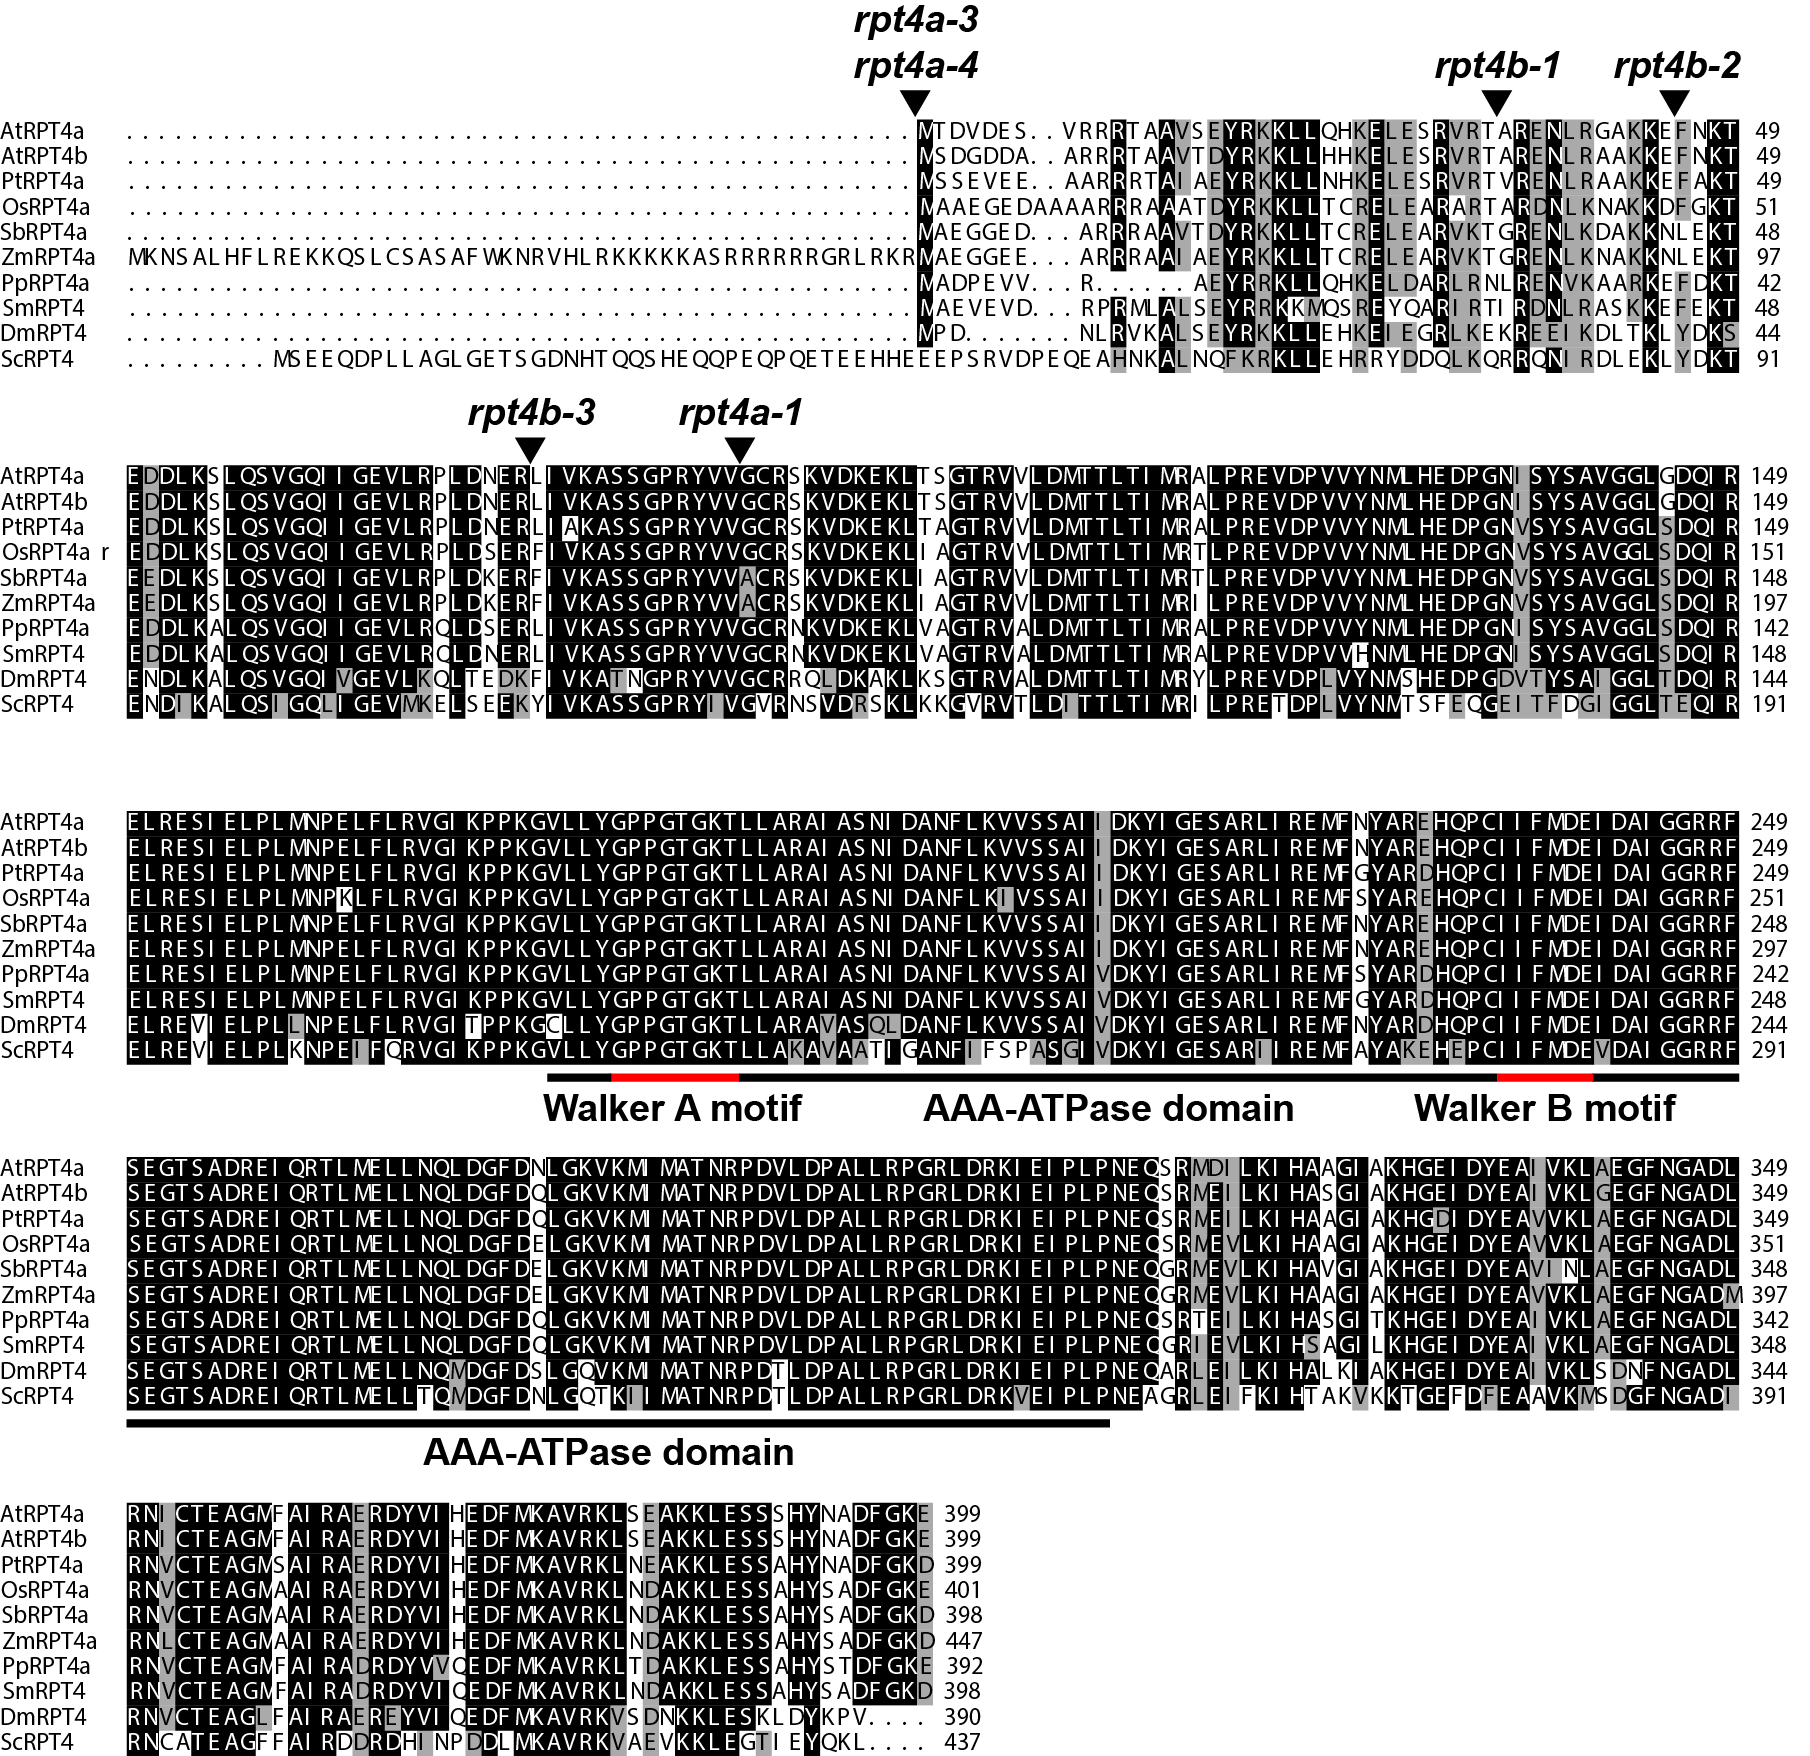
\includegraphics[width=\columnwidth]{Proteasome/suprpt4mut.png}
	\mycaption{Sequence Alignments of RPT4a and RPT4b}
	{Sequence Alignments of \textit{Arabidopsis} RPT4a RPT4b and related sequences was performed with ClustalW. Positions of T-DNA insertion mutants for both RPT4a and RPT4a were determined by sequencing T-DNA specific PCR products and are shown with black triangles. The AAA-ATPase domain is indicated with a black bar. The Walker A and B motifs contained in the AAA-ATPase domain are indicated in red. Species names are abbreviated as follows: At – \textit{Arabidopsis thaliana}, Pt – \textit{Populus trichocarpa}, Os – \textit{Oryza sativa}, Sb – \textit{Sorghum bicolor}, Zm- \textit{Zea mays}, Pp – \textit{Physcomitrella patens}, Sm – \textit{Selaginella moellendorffii}, Dm – \textit{Drosophila melanogaster}, Sc- \textit{Saccharomyces cerevisiae}.}
	\label{fig:suprpt4}
\end{figure}

\begin{figure}[ht]
	\centering
	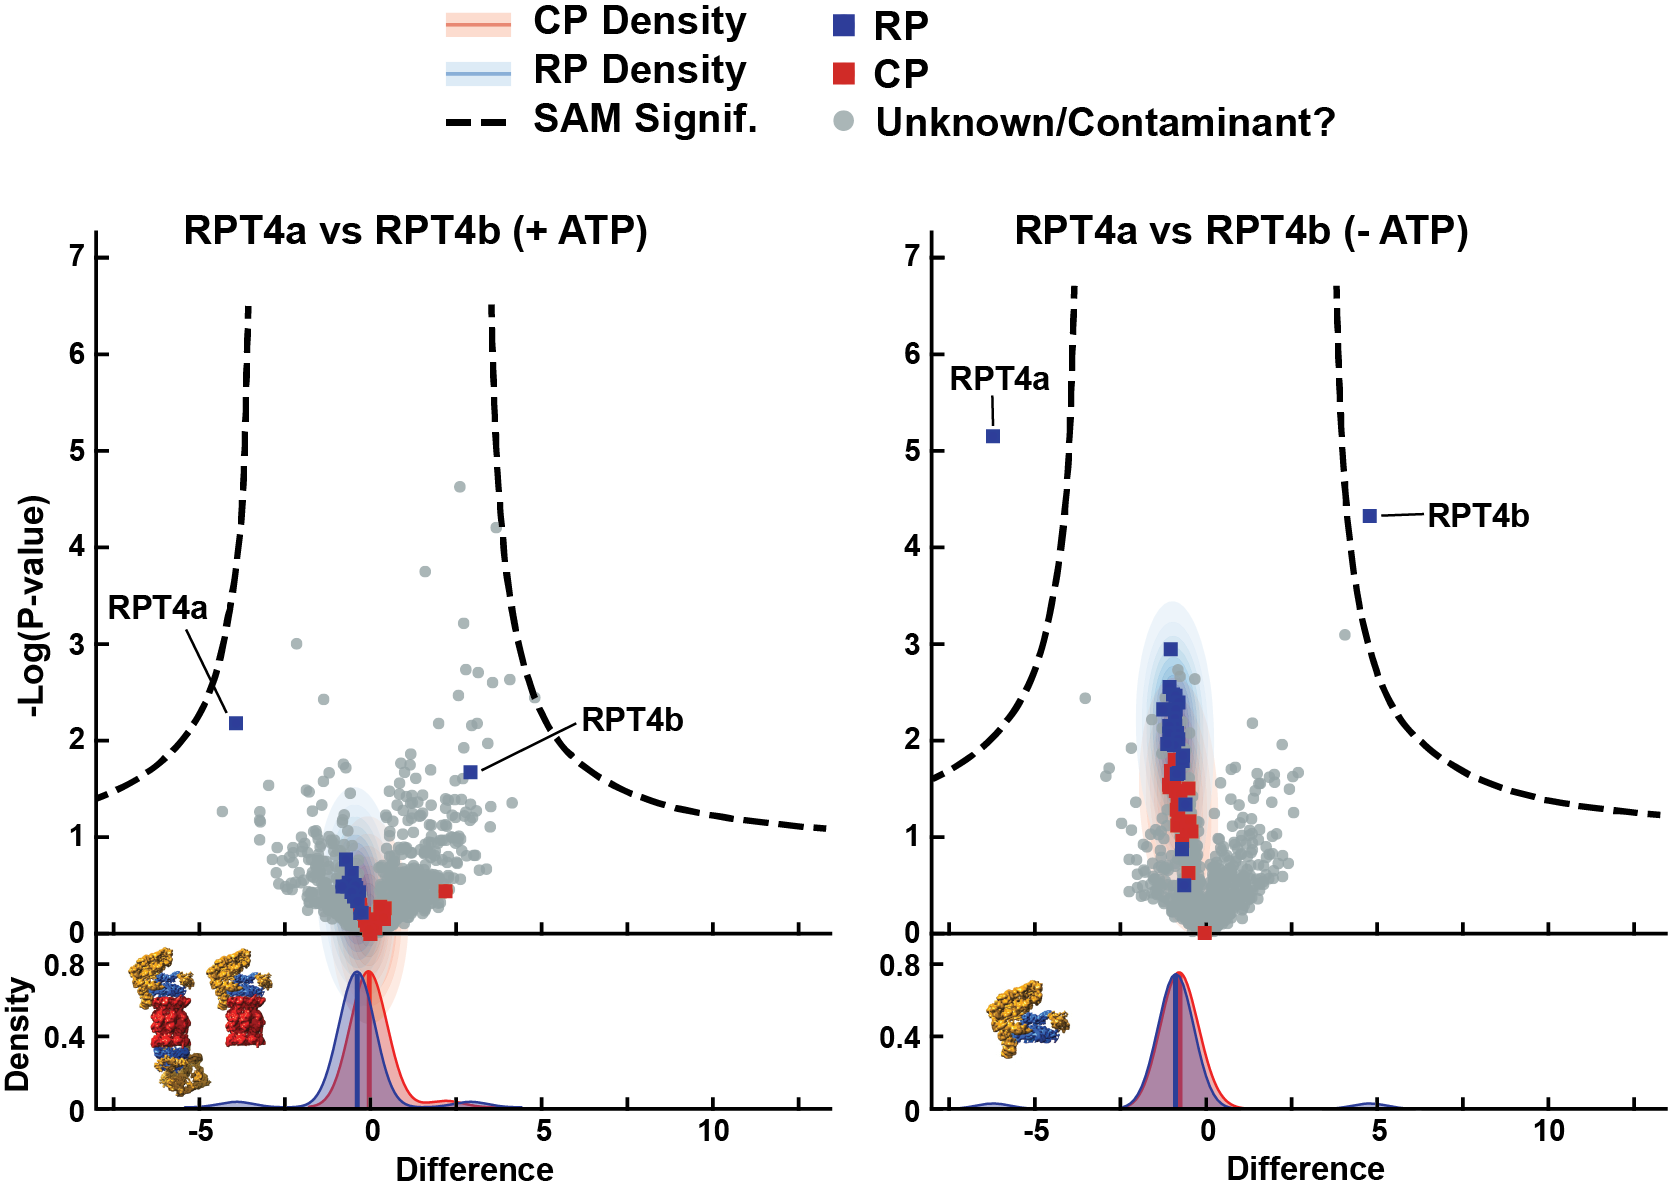
\includegraphics[width=\columnwidth]{Proteasome/supprpt4avsrpt4b.png}
	\mycaption{Volcano Plots Comparing Protein Profiles of Proteasome Affinity Purifications Based on RPT4a or RPT4b subunits in the presence (+) or absence (-) of ATP}
	{\textbf{(A)} In the presence of ATP, statistical analysis using significant analysis of microarray (SAM) test does not show enrichment for RPT4a in the RPT4a pulldown and RPT4b in the RPT4b pulldown. \textbf{(B)} In the absence of ATP, statistical analysis using a SAM test does show enrichment for RPT4a in the RPT4a pulldown and RPT4b in the RPT4b pulldown, but shows no other associations with central proteasome subunits or associated proteins. This suggests the complex assembles in a random fashion with respect to isoform incorporation.}
	\label{fig:suprpt4avsrpt4b}
\end{figure}




Figure S3 – Kernel Density Estimates (KDE) of the CP and RP distributions from label-free quantitative mass spectrometry show enrichment for the CP when purified via PAG1-FLAG, and for the RP when purified via FLAG-RPT4a/b. The X-axis shows difference in CP (red) or RP (blue) protein levels between affinity-purified samples and their respective mock affinity purification control, while the Y-axis is unit less with the area of each density corresponding to a total area of 1. Fold change (FC) CP over RP, or RP over CP was calculated based on the median of these distributions. Two \textit{p}-values, one for a median test, and another for a Kolmogorov-Smirnov test, are shown, which test for differences in median and overall distribution respectively. Cryo-EM structures of the sub-complexes likely to be enriched in each affinity purification are shown, with free CP (A) and RP (C and E) in the absence of ATP, and in the presence of ATP half capped and doubly capped proteasomes (B, D, and F) adapted from \citep{beck12} \textbf{(A)} The CP is enriched over 20 fold when performing an affinity purification with ATP omitted from the purification buffer as compared to the RP. \textbf{(B)} The CP is only enriched 1.5 fold when affinity purified in the presence of 20 mM ATP. \textbf{(C)} The RP as compared to the CP is enriched approximately 3.5 fold in samples that were purified via FLAG-RPT4a in the absence of ATP. \textbf{(D)} In the presence of 20 mM ATP this RP enrichment decreases to only 2 fold for RPT4a. \textbf{(E)} In the absence of ATP the RP is enriched approximately 3.5 fold in samples affinity purified from RPT4b. \textbf{(F)} Enrichment for the RP decreases to about 2 fold in the presence of 20 mM ATP.


Figure S4 – Multiple Sequence Alignment for UMP1. A Clustal Omega \citep{sievers14} sequence alignment of UMP1 from plants, yeast, and animals visualized with the program BOXSHADE. A heat map showing each combination of protein percent identity with respective values shown in each cell obtained from the resultant clustalo identity matrix. 

Figure S5 – Multiple Sequence Alignment for PBAC1. A Clustal Omega \citep{sievers14} sequence alignment of PBAC1 from plants, yeast (PBA1), and animals (PAC1) visualized with the program BOXSHADE. A heat map showing each combination of protein percent identity with respective values shown in each cell obtained from the resultant clustalo identity matrix. Species names are abbreviated as follows: A.th – \textit{Arabidopsis thaliana}, Z.ma – \textit{Zea mays}, Os – \textit{Oryza sativa}, M.tr – \textit{Medicago truncatula}, P.pa – \textit{Physcomitrella patens}, S.ec- \textit{Saccharomyces cerevisiae} K.la – {Kluyveromyces lactis}, E.go – \textit{Eremothecium gossypii}, D.ha – \textit{Debaryomyces hansenii}, D.me – \textit{Drosophila melanogaster}, X.la – \textit{Xenopus laevis}, D.re – \textit{Danio rerio}, M.mu – \textit{Mus musculus}, H.sa, \textit{Homo sapiens}.


Figure S6 – Multiple Sequence Alignment for PBAC2. A Clustal Omega \citep{sievers14} sequence alignment of PBAC2 from plants, yeast (PBA2), and animals (PAC2) visualized with the program BOXSHADE. A heat map showing each combination of protein percent identity with respective values shown in each cell obtained from the resultant Clustal Omega identity matrix. Species abbreviations are listed in Figure S5

Figure S7 – Multiple Sequence Alignment for PBAC3. A Clustal Omega \citep{sievers14} sequence alignment of PBAC3 from plants, yeast (PBA3), and animals (PAC3) visualized with the program BOXSHADE. A heat map showing each combination of protein percent identity with respective values shown in each cell obtained from the resultant Clustal Omega identity matrix. Species abbreviations are listed in Figure S5

Figure S8 – Multiple Sequence Alignment for PBAC4. A Clustal Omega \citep{sievers14} sequence alignment of PBAC4 from plants, yeast (PBA4), and animals (PAC4) visualized with the program BOXSHADE. A heat map showing each combination of protein percent identity with respective values shown in each cell obtained from the resultant Clustal Omega identity matrix. Species abbreviations are listed in Figure S5

Figure S9 – Multiple Sequence Alignment for PAP1. A Clustal Omega \citep{sievers14} sequence alignment of PAP1 visualized with the program BOXSHADE. A heat map showing each combination of protein percent identity with respective values shown in each cell obtained from the resultant Clustal Omega identity matrix. Species abbreviations are listed in Figure S5

Figure S10 – Full BiFC Panel and Controls. BiFC analysis showing both GFP channel and a merged bright-field and GFP channel. \textbf{(A)} A repeat of Figure 6D is shown for reference \textbf{(B)} Additional controls combining N-YFP and C-YFP with their respective N and C terminal YFP-fused PBAC1, PBAC2, PBAC3, and PAP1.

Figure S11 – Phylogenetic Analysis of PAP1 and PBAC1-4. Bayesian phylogenetic analysis of PAP1 and PBAC1-4 from sequence alignments shown in Figure S5-S9. Trees were generated with MrBayes \citep{ronquist12} and then visualized with FigTree. Nodes are color-coded with clade probabilities (probability of observing this grouping in the set of sampled trees), and a color key is shown on the right. Species names are abbreviated as follows: A.th – \textit{Arabidopsis thaliana}, Z.ma – \textit{Zea mays}, Os – \textit{Oryza sativa}, M.tr – \textit{Medicago truncatula}, P.pa – \textit{Physcomitrella patens}, S.ec- \textit{Saccharomyces cerevisiae} K.la – \textit{Kluyveromyces lactis}, E.go – \textit{Eremothecium gossypii}, D.ha – \textit{Debaryomyces hansenii}, D.me – \textit{Drosophila melanogaster}, X.la – \textit{Xenopus Laevis}, D.re – \textit{Danio rerio}, M.mu – \textit{Mus musculus}, H.sa, \textit{Homo sapiens}. \textbf{(A)} Phylogeny generated with all sequences from yeast, animals, and plants. Clear grouping is observed between the yeast, animal, and putative plant PBAC2 orthologs into a single clade. Grouping was observed for PBAC3 between the animal, and putative plant sequences; however, yeast PBAC3 was not found in this clade. Clear grouping is observed for PBAC4 between the animal, and putative plant sequences; however, yeast PBAC4 was not found in this clade. Animal, yeast, and plant PBAC1 did not clearly group, likely due to considerable sequence divergence. \textbf{(B)} Phylogeny generated when omitting the yeast sequences and only utilizing animal and plant sequences. Clear grouping is observed between the putative plant orthologs PBAC2-4 with their respective animal orthologs into separate clades. Animal PBAC1 does not group with the putative plant specific PBAC1 orthologs, likely due to considerable sequence divergence from animal PBAC1.

Table S1 – Oligonucleotide Primer Sequences Used in this Study. A table of primers used throughout this chapter is provided for reference.

Table S2 – Contaminants Removed from MaxQuant’s ProteinGroups.txt file. A list of common contaminants that were removed from MaxQuant’s ProteinGroups.txt file for the proteomics experiments involving PAG1-FLAG, and FLAG-RPT4a/b affinity purified proteasomes.  ATG Identifiers, Symbols and descriptions from The \textit{Arabidopsis} Information Resource v 10 (TAIR10) are provided.

Table S3 – Bioinformatic Analysis of PBAC1-4 and PAP1 Sequences. \textbf{(A)} InterProScan \citep{jones14} analysis of \textit{Arabidopsis} protein sequences for PBAC1-4 with InterProScan Signatures from both PFAM and Panther databases with their respective expectation-values (E-values) are shown for reference. While PBAC1 (previously identified as a likely ortholog for PAC1 \citep{kusmierczyk11}) contains a Proteasome Assembly Chaperone (PAC) 2 domain shown with a star, it is of considerably lower expectation-value (E-value) than PBAC2 which contains a Proteasome Assembly Chaperone (PAC) 2 domain. PBAC3 contains a PAC3 domain, and PBAC4 contains a PAC4 domain. PAP1 contains no domains of known function but does contain a conserved domain annotated in the Panther database \citep{mi05}. \textbf{(B)} Iterative PSI-BLAST Analysis was performed on NCBI’s non-redundant (nr) database using the human PAC1-4 sequences using the default parameters. PBAC1-4 were the top hits in \textit{Arabidopsis} for their respective PAC1-4 search sequences. ATG identifiers, RefSeq identifiers, Number of PSI-BLAST iterations, and expectation values (E-value) are listed for each analysis. PBAC1 required a second iteration to be identified, in which all sequences above the default expectation threshold were included in the second search.

Table S4 – Proteasome associated proteins identified after PAG1-based affinity purification under both plus and minus ATP Conditions. A table of proteins identified as significantly enriched at FDR 0.01 in the indicated affinity preparations.  Shown are the protein’s ATG identifiers, descriptions from \textit{The Arabidopsis Information Resource version 10} (TAIR10), symbols from TAIR10, average MS/MS count, average sequence coverage, fold change compared to control using the MaxLFQ value from MaxQuant, and \textit{p}-values obtained from the volcano plots in Figure 4A and B.

Table S5 – Proteasome associated proteins identified after RPT4a-based affinity purification under both plus and minus ATP conditions. A table of proteins identified as significantly enriched at FDR 0.01 in the indicated affinity preparations.  Shown are the protein’s ATG identifiers, descriptions from \textit{The Arabidopsis Information Resource version 10 (TAIR10)}, symbols from TAIR10, average MS/MS count, average sequence coverage, fold change compared to control using the MaxLFQ value from MaxQuant, and \textit{p}-values obtained from the volcano plots in Figure 4C and D.

Table S6 – Proteasome associated proteins identified after RPT4b-based affinity purification under both plus and minus ATP conditions. A table of proteins identified as significantly enriched at FDR 0.01 in the indicated affinity preparations.  Shown are the proteins ATG identifiers, descriptions from \textit{The Arabidopsis Information Resource version 10 (TAIR10)}, symbols from TAIR10, average MS/MS count, average sequence coverage, fold change compared to control using the MaxLFQ value from MaxQuant, and \textit{p}-values obtained from the volcano plots in Figure 4E and F.

Table S7 – dNSAF values determined by Morpheus Spectral Counter used to generate the heatmap in Figure 6C. Proteins as annotated in the heatmap are listed with each slice and treatment status as treated or untreated with MG132. dNSAF values as determined by Morpheus Spectral Counter \citep{gemperline16} are listed for each slice.

Table S8 –Fold Change dNSAF values comparing Slice 1 and Smear from Figure 6. Fold change values were calculated for both treated and untreated samples by dividing the dNSAF values for Smear / Slice 1. \#DIV/0! Is listed as a divide by zero error, in that those proteins were detected in the smear but not in Slice 1. Larger values were color coded by red in Microsoft Excel, and smaller values were color coded by blue.
